% -*- TeX-master: "main"; fill-column: 72 -*-

\section{Proposed syntax and semantics}
\label{syntax}

In this section, we define the syntax and semantics of the Render package for SBML Level~3 
Version~1.  We expound on the various
data types and constructs defined in this package, then in \sect{examples},
we provide complete examples of using the constructs in example SBML
models.

\subsection{Namespace URI and other declarations necessary for using this
package}
\label{xml-namespace}

Every SBML Level~3 package is identified uniquely by an XML namespace URI.
For an SBML document to be able to use a given SBML Level~3 package, it
must declare the use of that package by referencing its URI.  The following
is the namespace URI for this version of the Render
package for SBML Level~3 Version~1:
\begin{center}
\uri{http://www.sbml.org/sbml/level3/version1/render/version1}
\end{center}

In addition, SBML documents using a given package must indicate whether understanding the package is required for complete mathematical interpretation of a model, or whether the package is optional.  This is done using the attribute \token{required} on the \token{<sbml>} element in the SBML document.  For the \RenderPackage, the value of this attribute must be set to \val{false}.

The following fragment illustrates the beginning of a typical SBML model
using SBML Level~3 Version~1 and this version of the Rendering package (note, that the Layout package is also needed):

\begin{example}
<?xml version="1.0" encoding="UTF-8"?>
 <sbml xmlns="http://www.sbml.org/sbml/level3/version1/core" level="3" version="1"
   xmlns:layout="http://www.sbml.org/sbml/level3/version1/layout/version1" layout:required="false"
   xmlns:render="http://www.sbml.org/sbml/level3/version1/render/version1" render:required="false"
	>
	
\end{example}


Originally the layout and render extension have been developed for use with SBML Level 2 files, there the information was stored in annotations to SBML models, layout lists and layouts.
The namespace for these version of the SBML render extension for SBML level 2 is: 

\begin{center}
\uri{http://projects.eml.org/bcb/sbml/render/level2}
\end{center}

an example on how to use the render extension in this context would look like this: 

\begin{example}
<?xml version="1.0" encoding="utf-8"?>
<sbml xmlns="http://www.sbml.org/sbml/level2" level="2" version="1">
  <model id="model1" name="Model with L2 Render Annotation">
    <annotation>
      <listOfLayouts xmlns="http://projects.eml.org/bcb/sbml/level2">
        <layout id="layout1">
          <annotation>
            <listOfRenderInformation xmlns="http://projects.eml.org/bcb/sbml/render/level2">
							...
            </listOfRenderInformation>
          </annotation>
					...
        </layout>
				...
      </listOfLayouts>
			...
    </annotation>
		...
  </model>
</sbml>
\end{example}


\begin{figure}[h!]
  \centering
  % Requires \usepackage{graphicx}
  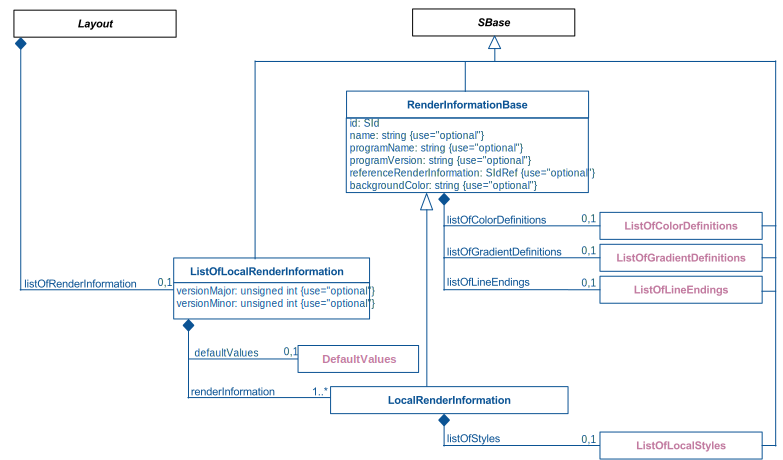
\includegraphics[width=\textwidth]{images/render-layout-uml}\\
  \caption{A UML representation of the \RenderPackage. Derived from \SBase, the \Render classes inherit support for constructs such as SBML \Notes and \Annotation's. See \ref{conventions} for conventions related to this figure. The individual classes are further discussed in the text.}
  \label{fig:Render_uml}
\end{figure}

\subsection{Primitive data types}
\label{primtypes}

Section~3.1 of the \sbmlthreecore specification defines a number of primitive
data types and also uses a number of XML Schema 1.0 data types~\citep{biron:2000}.
More specifically we make use of \primtype{integer}, \primtype{double},
\primtype{string}, \primtype{SId} and \primtype{SIdRef}. 
In addition we make use of
four new primitives \primtype{StyleType}, \primtype{GradientSpreadMethod}, 
\primtype{FillRule}, \primtype{VTextAnchors}, \primtype{HTextAnchors},  
\primtype{FontFamily}, \primtype{FontWeight} and \primtype{FontStyle}.
%see \ref{fig:Render_uml} for the interrelation between these entities.

The \primtype{SId} type is used as the data type for the identifiers of \RenderInformation
(\ref{renderinformation-class}), \Curve (\ref{curve-class}),  and \Polygon
(\ref{polygon-class}) classes. 
%In the Render package the \ListOfObjectives has an
%attribute of type \primtype{SIdRef} that is used to refer to an `active' \Objective.

\subsubsection{The \primtype{StyleType} type}
\label{style-type}
The type \primtype{StyleType} is used by \LocalStyle and \GlobalStyle elements, in order
to apply a particular \Style to a \GraphicalObject. This is done via the \token{typeList}
that uses the \primtype{StyleType} as its data type. 

A valid \primtype{StyleType} instance is a combination of one or more of the following 
values separated by white spaces:

\begin{itemize}
 \item \val{COMPARTMENT\-GLYPH},
 \item \val{SPECIES\-GLYPH},
 \item \val{REACTION\-GLYPH}, 
 \item \val{SPECIES\-REFERENCE\-GLYPH},
 \item \val{TEXT\-GLYPH}, 
 \item \val{GENERAL\-GLYPH}, 
 \item \val{GRAPHICAL\-OBJECT} and 
 \item \val{ANY}
\end{itemize}


\subsubsection{The \primtype{GradientSpreadMethod} type}
\label{gradientspreadmethod-type}
The type \primtype{GradientSpreadMethod} is being used by \GradientBase elements to decide how 
gradients propagate over the whole element they are applied to. It is an enumeration consisting 
of the following three values called \texttt{pad}, \texttt{reflect} or \texttt{repeat}:

\begin{itemize}
 \item {\texttt{pad}:} the gradient color at the
endpoint of the vector defines how the gradient is continued beyond that point (default value).
 \item {\texttt{reflect}:} the gradient continues from end to start and
then from start to end again and again.
 \item {\texttt{repeat}:} the gradient pattern is repeated from start to end over and over again.
\end{itemize}

\begin{figure}[!ht]
\begin{center}
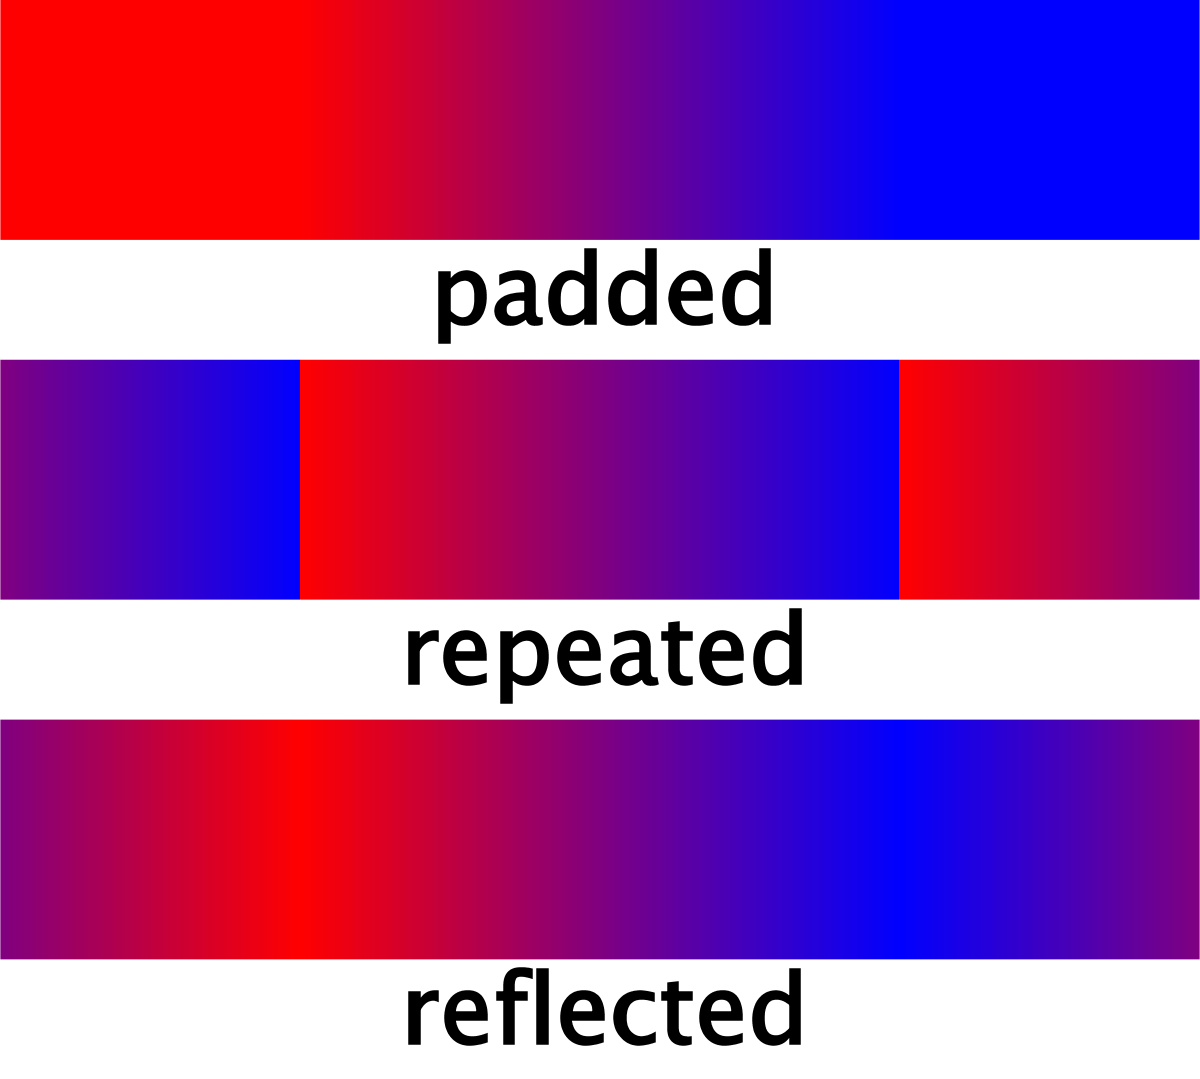
\includegraphics[scale=0.18]{figures/SVG_spreadMethod.png}
\end{center}
\caption{example of different SVG spreadMethod values}
\label{SVG:spreadMethod}
\end{figure}

\subsubsection{The \primtype{FillRule} type}
\label{fillrule-type}
The type \primtype{FillRule} describes how a surface created by connecting 
points on a \Polygon are to be filled when rendered. Allowed values for a valid instance of type \primtype{FillRule} are:

\begin{itemize}
 \item \token{nonzero} (default) or
 \item \token{evenodd}.
\end{itemize}

For a detailed description on how those attributes work in detail, we would like to refer you to the corresponding documentation in the SVG specification. 

\subsubsection{The \primtype{VTextAnchor} type}
\label{vtextanchor-type}
The type \primtype{VTextAnchor} allows to specify how text elements are to be
vertically aligned within their bounding box. This enumeration has the following allowed values: 

\begin{itemize}
 \item \token{top},
 \item \token{middle},
 \item \token{bottom} and
 \item \token{baseline}
\end{itemize}

Examples for the alignments can be found in the figures below. 

\begin{figure}[!ht]
\begin{center}
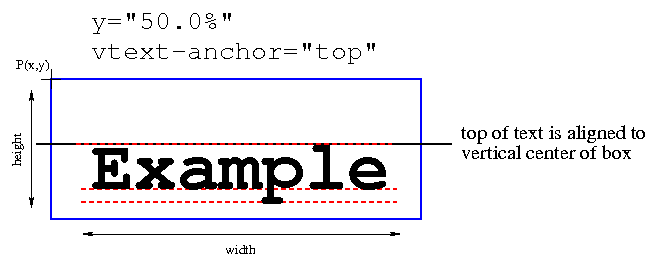
\includegraphics[scale=0.60]{figures/VerticalTextPlacement2}
\end{center}
\caption{vertical text alignment \token{top}}
\label{VerticalTextPlacement2}
\end{figure}

\begin{figure}[!ht]
\begin{center}
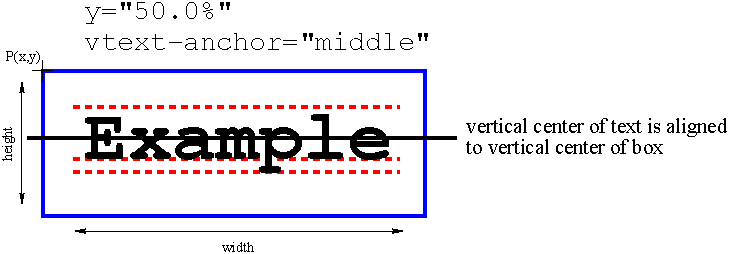
\includegraphics[scale=0.60]{figures/VerticalTextPlacement3}
\end{center}
\caption{vertical text alignment \token{bottom}}
\label{VerticalTextPlacement3}
\end{figure}

\begin{figure}[!ht]
\begin{center}
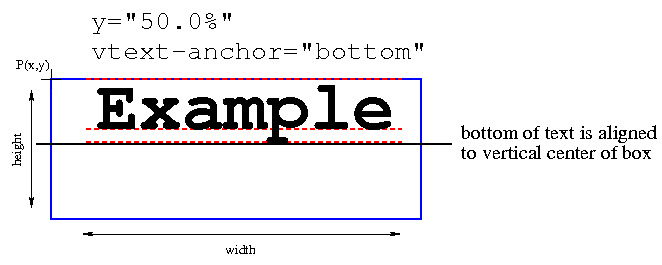
\includegraphics[scale=0.60]{figures/VerticalTextPlacement4}
\end{center}
\caption{vertical text alignment \token{middle}}
\label{VerticalTextPlacement4}
\end{figure}

\begin{figure}[!ht]
\begin{center}
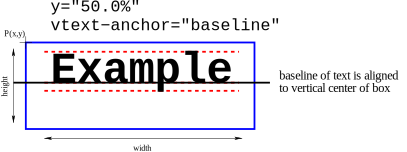
\includegraphics[scale=0.60]{figures/VerticalTextPlacement5}
\end{center}
\caption{vertical text alignment \token{baseline}}
\label{VerticalTextPlacement5}
\end{figure}


\subsubsection{The \primtype{HTextAnchor} type}
\label{htextanchor-type}
The type \primtype{HTextAnchor} defines analog to the \primtype{VTextAnchor}
the horizontal alignment of text elements. This enumeration can use the following values: 

\begin{itemize}
 \item \token{start},
 \item \token{middle} and
 \item \token{end}
\end{itemize}

The figures below demonstrate the different horizontal alignment options.

\begin{figure}[!ht]
\begin{center}
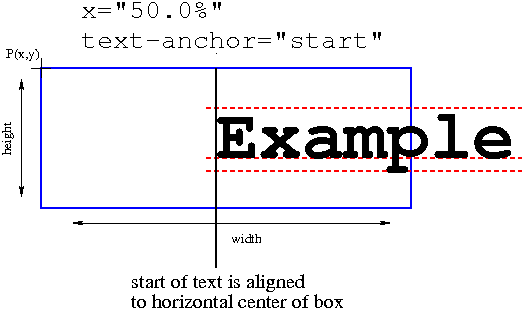
\includegraphics[scale=0.60]{figures/HorizontalTextPlacement_Start}
\end{center}
\caption{horizontal text alignment \token{start}}
\label{HorizontalTextPlacement_Start}
\end{figure}

\begin{figure}[!ht]
\begin{center}
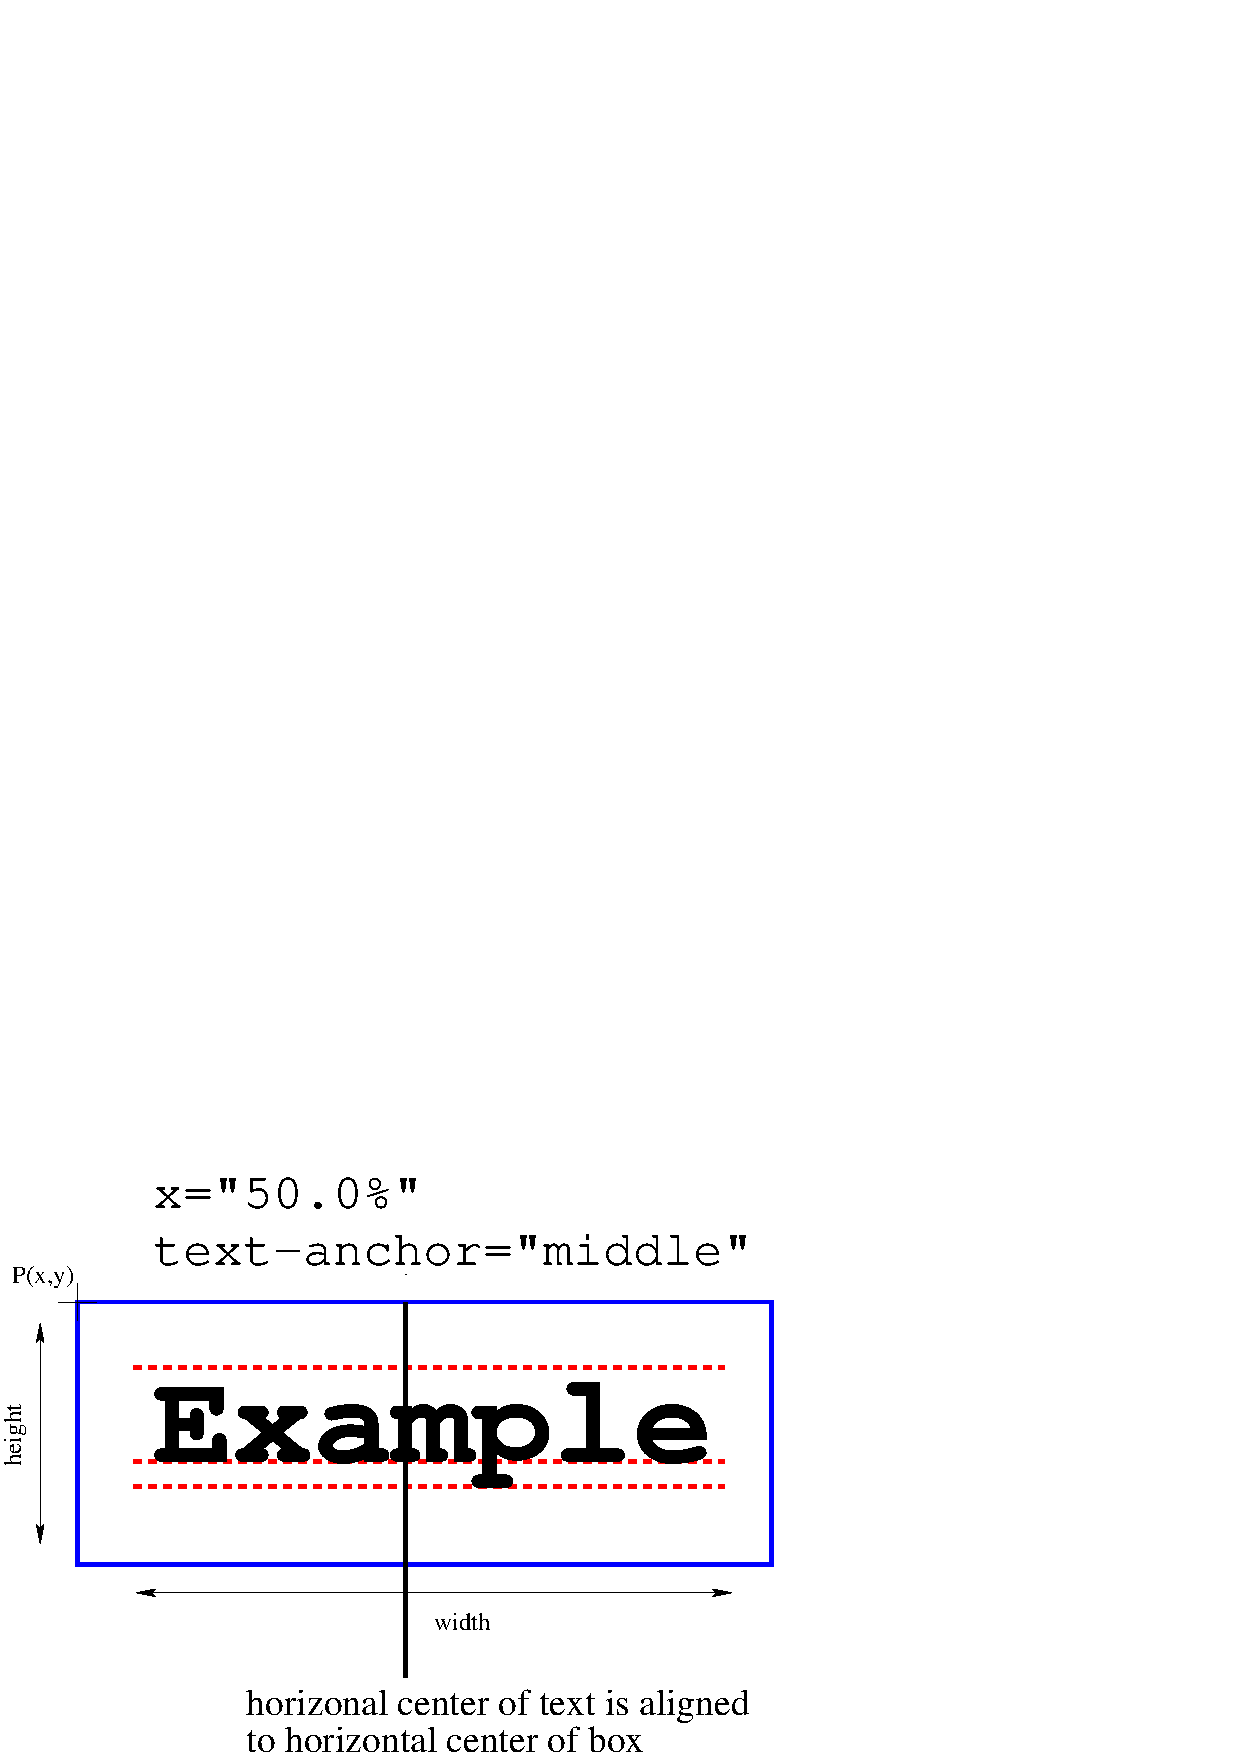
\includegraphics[scale=0.60]{figures/HorizontalTextPlacement_Middle}
\end{center}
\caption{horizontal text alignment \token{middle}}
\label{HorizontalTextPlacement_Middle}
\end{figure}

\begin{figure}[!ht]
\begin{center}
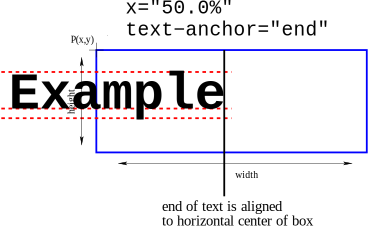
\includegraphics[scale=0.60]{figures/HorizontalTextPlacement_End}
\end{center}
\caption{horizontal text alignment \token{end}}
\label{HorizontalTextPlacement_End}
\end{figure}


\subsubsection{The \primtype{FontFamily} type}
\label{fontfamily-type}
The type \primtype{FontFamily} gives a hint, what font is to be used when
rendering \Text elements. This type extends the type \primtype{string}, 
pre-defined are: 

\begin{itemize}
 \item \token{serif},
 \item \token{sans-serif} and
 \item \token{monospace}
\end{itemize}

However, in actual applications, the \primtype{FontFamily}
is usually used to store the name of the font the writing application used. It has not been a issue for reading applications to find a similar font. 

\subsubsection{The \primtype{FontWeight} type}
\label{fontweight-type}
The type \primtype{FontWeight} indicates whether the font is to be used in its normal form, or in its bold form. Consequently, the only values allowed for this enumeration are: 

\begin{itemize}
 \item \token{bold} and
 \item \token{normal} 
\end{itemize}

\subsubsection{The \primtype{FontStyle} type}
\label{fontstyle-type}
The type \primtype{FontStyle} determines whether a font is to be
drawn italic or normal. Thus the only allowed values are:

\begin{itemize}
 \item \token{italic} and
 \item \token{normal} 
\end{itemize}

\subsection{General features}

The render extension provides two locations where styles can be defined. First 
each layout can have its own set of render information located in the 
annotation of the \Layout element (local render information). 
Second, a set of global render information objects 
located in the annotation of the \ListOfLayouts element can be defined. 

It is important to note that each layout can have more than one 
set of local render information and that it is 
also possible to define more then one global style. Each style can also 
reference another style that complements it, this way the user can create 
styles that are based on other styles. In contrast to local styles, the global styles can not 
reference individual layout elements by an id, they can only define role based or 
type based styles.

\subsubsection{Positions and sizes}

Positions and sizes for render elements can be specified as a combination of absolute 
values where the default unit is pt (1/72 inch) 
and relative values in \% where the \% symbol has to be added to 
the value. Each coordinate can have zero or one relative component and zero or one absolute component.
For example to specify a coordinate that is 5 points left of the right edge of the current view port the
user could specify $-5+100\%$. 

In order to make parsing of coordinate information easier, the absolute 
component has to be specified before the relative component. If the absolute component is 0.0, only the relative part has to be specified.
All values are relative to the bounding box of the corresponding 
element in the layout. This bounding box basically specifies a canvas for the 
render elements to be drawn on.

When applying transformations to elements with relative values, the relative values have to be converted to absolute values first.



\subsubsection{Uniqueness of ids}
Since local and global render information objects can reference other render information objects, programs creating
render information need to make sure that all the ids are unique within the reference history. In other words, a 
render information object that references another render information object must make sure that none of its ids is equal
to an id in any of the directly or indirectly referenced render information objects. 

An exception to this rule is to create e.g. a color definition with the same id as the color definition in a referenced style
in this case interpreting programs can assume that this color definition is supposed to override the color definition  with the
same name in the referenced render information object. Likewise it is also possible to override a color definition with a 
gradient and vice versa. Line ending definitions on the other hand can only be replaced by other line ending definitions.

\subsection{The extended \ListOfLayouts class}
The \ListOfLayouts class of the Layout package is extended by an optional element \token{listOf\-Global\-Render\-Information} of 
class \ListOfGlobalRenderInformation. 

\subsubsection{The \ListOfGlobalRenderInformation class}
\label{listofrenderinformation-class}
The \ListOfGlobalRenderInformation class is derived from \SBase and defines two optional attributes
\token{versionMajor} and \token{versionMinor}. It contains one or more elements of type \GlobalRenderInformation.

\begin{figure}[!ht]
%\includegraphics[scale=0.5]{figures/SBase}
\footnotesize{
\renewcommand{\arraystretch}{1.3}
\begin{tabular}{|lcl|}
\hline
\multicolumn{3}{|c|}{\ListOfGlobalRenderInformation inherits from \SBase}\\
\hline
versionMajor & : & unsigned int \\ \hline           
versionMinor & : & unsigned int \\ \hline           
renderInformation & : & GlobalRenderInformation[$1..\ast$]\\ \hline           
\end{tabular}
}
\renewcommand{\arraystretch}{1.0}

\end{figure}
\vspace*{0.25cm}

\paragraph{The \token{versionMajor} and \token{versionMinor} attributes }
The \token{versionMajor} attribute of type \primtype{int} specifies the major version of the render information. 
Major version do not have to be backwards compatible to any lower major version of the render specification.
The \token{versionMinor} attribute of type \primtype{int} specifies the minor version of the render information. 
All minor versions within a major version have to be compatible.

\subsection{The extended \Layout class}
The \Layout class of the Layout package is extended by an optional element \token{listOf\-Render\-Information} 
of class \ListOfLocalRenderInformation.

\subsubsection{The \ListOfLocalRenderInformation class}
\label{listoflocalrenderinformation-class}
The \texttt{listOf\-Render\-Information} of type \ListOfLocalRenderInformation can contain a list of one or more 
\texttt{render\-Information} elements of type \LocalRenderInformation.
In addition to the list of local render information objects, the \ListOfLocalRenderInformation defines two optional attributes
\token{versionMajor} and \token{versionMinor}. The \ListOfLocalRenderInformation class is derived from \SBase.

\begin{figure}[!ht]
\footnotesize{
\renewcommand{\arraystretch}{1.3}
\begin{tabular}{|lcl|}
\hline
\multicolumn{3}{|c|}{\ListOfLocalRenderInformation inherits from \SBase}\\
\hline
versionMajor & : & unsigned int \\ \hline           
versionMinor & : & unsigned int \\ \hline           
renderInformation & : & LocalRenderInformation[$1..\ast$] \\ \hline           
\end{tabular}
}
\renewcommand{\arraystretch}{1.0}

\label{UML:ListOfLocalRenderInformation}
\end{figure}
\vspace*{0.25cm}

\paragraph{The \token{versionMajor} and \token{versionMinor} attributes }
The \token{versionMajor} attribute of type \primtype{int} specifies the major version of the render information. 
Major version do not have to be backwards compatible to any lower major version of the render specification.
The \token{versionMinor} attribute of type \primtype{int} specifies the minor version of the render information. 
All minor versions within a major version have to be compatible.

\subsection{The extended \GraphicalObject class}
The \Render Package extends the Layout \GraphicalObject class by an 
additional attribute \token{objectRole}. This attribute specifies with 
which \Style the object should be rendered.

\subsection{Render Information}
\label{renderinformation-class}
The render information classes hold all information about the rendering. This
information is kept in three classes: \RenderInformationBase, the base class with 
common features; \GlobalRenderInformation a class applying to types and roles of 
elements; and \LocalRenderInformation that additionally can be applied to individual
Layout elements.

\subsubsection{The \RenderInformationBase class}
\label{renderinformation-base-class}
This abstract class, derived from \SBase, holds all information common to both local and global render 
information objects. It is specified by the required attribute \token{id} and the 
optional attributes \token{name}, \token{programName}, \token{programVersion}, 
\token{referenceRenderInformation} and \token{backgroundColor}. Additionally it may
hold a \ListOfColorDefinitions, \ListOfGradientDefinitions and / or \ListOfLineEndings.

\begin{figure}[!ht]
%\includegraphics[scale=0.5]{figures/SBase}
\footnotesize{
\renewcommand{\arraystretch}{1.3}
\begin{tabular}{|lcl|}
\hline
\multicolumn{3}{|c|}{\RenderInformationBase inherits from \SBase}\\
\hline
id & : & SId \\
name & : & string \{use="optional"\}\\
programName & : & string \{use="optional"\}\\
programVersion & : & string \{use="optional"\}\\
referenceRenderInformation & : & string \{use="optional"\}\\
backgroundColor & : & string \{use="optional" default="\#FFFFFFFF" \}\\
listOfColorDefinitions & : & ListOfColorDefinitions \{use="optional"\}\\
listOfGradientDefinitions & : & ListOfGradientDefinitions \{use="optional"\}\\
listOfLineEndings & : & ListOfLineEndings \{use="optional"\}\\
\hline           
\end{tabular}
}
\renewcommand{\arraystretch}{1.0}

\label{UML:RenderInformationBase}
\end{figure}
\vspace*{0.25cm}
\paragraph{The \token{id} attribute}
The \token{id} attribute is of type \primtype{SId} like the ids 
in SBML. It is used to give the \token{renderInformation} element a unique id 
through which it can be referenced from other render information objects. 

\paragraph{The \token{name} attribute}
The optional attribute \token{name} of type \primtype{string} gives a 
render information object a more user friendly name that can be displayed 
in programs.

\paragraph{The \token{programName} and  \token{programVersion} attribute}
The attributes \token{programName} and \token{programVersion} are optional attributes of 
type \primtype{string} and can be used to store information about the program 
that created the render information. 

\paragraph{The \token{referenceRenderInformation} attribute}
Another optional attribute called \token{reference\-Render\-Information} of type
\primtype{SIdRef} can be used to specify the id of another local or global render information object 
that complements the current render information object. So if a program can 
find no fitting render information in the current render information object, it 
can go on to the one referenced and see if it can find fitting information 
there. In order to avoid loops, only render information objects that have 
already been defined before may be referenced. So local render information 
objects may reference any global render information object as well as any local 
render information object that has already been defined and belongs to the same layout. 

\paragraph{The \token{backgroundColor} attribute}
In addition to those five attributes, the \RenderInformationBase object has an optional
attribute called \token{backgroundColor} which defines the background color for rendering the layout.

\paragraph{The \ListOfColorDefinitions element}
\label{listofcolordefinitions-class}
The element called \texttt{listOf\-Color\-Definitions} is of type \ListOfColorDefinitions. It may be 
used to predefine a set of colors to be referenced in styles. If present it must contain one or more
elements of class \ColorDefinition.

\paragraph{The \ListOfGradientDefinitions element}
\label{listofgradientdefinitions-class}
The element  \texttt{listOf\-Gradient\-Definitions}  of type \ListOfGradientDefinitions
contains linear and radial gradients to be referenced in styles. How colors and gradients can
be defined is explained in the section called "Colors and gradients". 

\paragraph{The \ListOfLineEndings element}
\label{listoflineendings-class}
The third element is called \texttt{list\-Of\-Line\-Endings} and it is used to define a
set of line endings that can be applied to path objects. This is explained in
more detail in the section called "Line endings". 

\subsubsection{The \LocalRenderInformation class}
\label{local-renderinformation-class}
The element \texttt{render\-Information} of type \LocalRenderInformation is the primary container that holds the render information for a \Layout instance. The \LocalRenderInformation inherits from \RenderInformationBase.

\begin{figure}[!ht]
%\includegraphics[scale=0.5]{figures/SBase}
\footnotesize{
\renewcommand{\arraystretch}{1.3}
\begin{tabular}{|lcl|}
\hline
\multicolumn{3}{|c|}{\LocalRenderInformation inherits from \RenderInformationBase}\\
\hline
listOfStyles & : & ListOfLocalStyles \{use="optional"\}\\
\hline           
\end{tabular}
}
\renewcommand{\arraystretch}{1.0}

\label{UML:LocalRenderInformation}
\end{figure}
\vspace*{0.25cm}


The \LocalRenderInformation class extends the \RenderInformationBase class by one element \texttt{list\-Of\-Styles}.

\paragraph{The \ListOfLocalStyles class}
\label{listoflocalstyles-class}
The element \texttt{list\-Of\-Styles} of type \ListOfLocalStyles can hold one or more \texttt{style} elements of type \LocalStyle.


\subsubsection{The \GlobalRenderInformation class}
\label{global-renderinformation-class}
Global render information is specified very similar to local render information 
there are only some slight differences that one has to be aware of. Global 
render information is stored in an element called 
\token{listOf\-Global\-Render\-Information} which contains one ore more 
\token{renderInformation} elements of type \GlobalRenderInformation.

The attributes and elements of \GlobalRenderInformation objects and 
\LocalRenderInformation objects are the same. The only difference here is the 
fact that \GlobalRenderInformation objects may only reference ids of other 
\GlobalRenderInformation objects in their 
\token{referenceRenderInformation} attribute. 

The \texttt{listOf\-Styles} element of the \GlobalRenderInformation object contains 
one or more \texttt{style} elements but this time these are of type 
\GlobalStyle. 

  
\begin{figure}[!ht]
\footnotesize{
\renewcommand{\arraystretch}{1.3}
\begin{tabular}{|lcl|}
\hline
\multicolumn{3}{|c|}{\GlobalRenderInformation inherits from \RenderInformationBase}\\
\hline
listOfStyles & : & ListOfGlobalStyles \{use="optional"\}\\
\hline           
\end{tabular}
}
\renewcommand{\arraystretch}{1.0}

\label{UML:GlobalRenderInformation}
\end{figure}
  

\vspace{0.25cm}
{\large
  {\bf
example:
}
}

{\footnotesize
\begin{example}
<listOfLayouts xmlns="http://projects.eml.org/bcb/sbml/level2"
         xmlns:xsi="http://www.w3.org/2001/XMLSchema-instance">
  <annotation>
    <listOfGlobalRenderInformation 
          xmlns="http://projects.eml.org/bcb/sbml/render/version1_0_0">
      <renderInformation id="FancyRenderer_GlobalDefault" 
                         name="default global style" 
                         programName="FancyRenderer" 
                         programVersion="0.1.1">
        <listOfColorDefinitions>
             ...
        </listOfColorDefinitions>
        <listOfGradientDefinitions>
             ...
        </listOfGradientDefinitions>
        <listOfLineEndings>
             ...
        </listOfLineEndings>
        <listOfStyles>
             ...
        </listOfStyles>
      </renderInformation>
    </listOfGlobalRenderInformation>
  </annotation>
</listOfLayouts>
\end{example}
}

\subsection{Styles}
\label{style-class}

\subsubsection{The \LocalStyle class}
\label{localstyle-class}
A \LocalStyle object has an attribute called \token{id} that uniquely identifies it. It also has an optional \token{roleList} attribute which lists all the roles 
the style applies to and it can have a \token{typeList} attribute which lists 
all the element types the style applies to. The valid types for the 
\token{typeList} attribute are a combination of one or more of the following 
values separated by white spaces:

\begin{itemize}
 \item COMPARTMENT\-GLYPH,
 \item SPECIES\-GLYPH,
 \item REACTION\-GLYPH, 
 \item SPECIES\-REFERENCE\-GLYPH
 \item TEXT\-GLYPH, 
 \item GENERAL\-GLYPH, 
 \item GRAPHICAL\-OBJECT and 
 \item ANY
\end{itemize}

The \token{ANY} keyword specifies that this styles applies to any type of glyph and 
would be equivalent to listing all the other keywords. Concerning the valid 
keywords for the \token{roleList} attribute we had thought about taking those 
from some kind of controlled vocabulary. Preferably, this would be some kind of 
ontology like SBO. The specifics of this will have to be discussed with other 
interested parties. 

For the time being, all layout objects derived from \GraphicalObject
will get an additional attribute called \token{objectRole}. This attribute can be used
to specify a string that specifies the role of the given object. If the same string appear
s in the \token{roleList} of some render information object, the render information 
applies to the object, but only if there is no render information object that is more
specific (see "Style resolution" and "Role resolution" below). 

\LocalStyle objects can have one more optional attribute 
which is called \texttt{idList}. This is simply a list of ids of layout objects the style applies to.

The only sub element of a style is a \texttt{g} element which specifies how the 
element(s) covered by the \token{idList}, \token{roleList} and \token{typeList} are to be rendered. The 
details of this element are described in the section about grouping.
  






\begin{figure}[!ht]
%\includegraphics[scale=0.5]{figures/SBase}
\footnotesize{
\renewcommand{\arraystretch}{1.3}
\begin{tabular}{|lcl|}
\hline
\multicolumn{3}{|c|}{\ListOfLocalStyles inherits from \SBase}\\
\hline
style & : & LocalStyle[$1..\ast$] \\ \hline           
\end{tabular}
}
\renewcommand{\arraystretch}{1.0}

\label{UML:ListOfLocalStyles}
\end{figure}
\vspace*{0.25cm}

\begin{figure}[!ht]
\footnotesize{
\renewcommand{\arraystretch}{1.3}
\begin{tabular}{|lcl|}
\hline
\multicolumn{3}{|c|}{\LocalStyle inherits from \Style}\\
\hline
idList & : & string[$1..\ast$] \{use="optional"\}\\ \hline           
\end{tabular}
}
\renewcommand{\arraystretch}{1.0}

\label{UML:LocalStyle}
\end{figure}
\vspace*{0.25cm}


{\large
{\bf
example:
}
}

{\footnotesize
\begin{example}
<listOfLayouts xmlns="http://projects.eml.org/bcb/sbml/level2"
         xmlns:xsi="http://www.w3.org/2001/XMLSchema-instance">
  <layout id="Layout_1">
    <annotation>
      <listOfRenderInformation 
           xmlns="http://projects.eml.org/bcb/sbml/render/version1_0_0">
        <renderInformation id="FancyRenderer_Default" 
        	                   name="default style" 
                           programName="FancyRenderer" 
                           programVersion="0.1.1">
          <listOfColorDefinitions>
            <colorDefinition ... />
                  ...
          </listOfColorDefinitions>
          <listOfGradientDefinitions>
            <linearGradient ... >
            	    ...
            </linearGradient>
            <radialGradient ... >
            	    ...
            </radialGradient>
                  ...
          </listOfGradientDefinitions>
          <listOfLineEndings>
               ...
          </listOfLineEndings>
          <listOfStyles>
            <style id="CompartmentGlyphStyle" typeList="COMPARTMENTGLYPH">
              <g ...>
                ...
              </g>
            </style>
             ...
          </listOfStyles>
        </renderInformation>
      </listOfRenderInformation>
    </annotation>
       ...
  </layout>
</listOfLayouts>
\end{example}
}

\subsubsection{The \GlobalStyle class}
\label{globalstyle-class}
The \GlobalStyle data type is also very similar to the \LocalStyle 
data type but the \GlobalStyle does not have an 
\token{idList} attribute since referencing individual ids from a layout does 
not make sense for a global render information object.
Otherwise global and local render information is specified in the same way.

\begin{figure}[!ht]
\footnotesize{
\renewcommand{\arraystretch}{1.3}
\begin{tabular}{|lcl|}
\hline
\multicolumn{3}{|c|}{\Style inherits from \SBase}\\
\hline
id & : & SId \{use="optional"\}\\ \hline           
roleList & : & string[$1..\ast$] \{use="optional"\}\\ \hline           
typeList & : & string[$1..\ast$] \{use="optional"\}\\ \hline           
g & : & Group \\ \hline           
\end{tabular}
}
\renewcommand{\arraystretch}{1.0}

\label{UML:Style}
\end{figure}




\subsection{Colors and gradients}    

\subsubsection{The \ColorDefinition class}
\label{colordefinition-class}

Although, it is possible to specify the color for a graphical primitive
directly, colors and especially gradients can be specified in a so called
\texttt{listOf\-Color\-Definitions} and \texttt{listOf\-Gradient\-Definitions} element
which are sub elements of the \RenderInformation data type.
The \texttt{listOf\-Color\-Definitions} element holds one or more elements called
\texttt{colorDefinition} of type \ColorDefinition. The \ColorDefinition data type
is derived from \SBase and has two additional attributes. One \token{id}
attribute which uniquely identifies the \ColorDefinition object within a
\RenderInformation object and an attribute called \token{value} which holds a
color value.

Color values are specified as a 6 to 8 digit hex string which defines the RGBA 
value of the color. If only the first six digits for the RGB value are given, 
the alpha value is assumed to be 0xFF which means that the color is totally 
opaque. Instead of specifying a color value, the value '\texttt{none}' can be given which is equal to 
no drawing at all. To specify '\texttt{none}' for the \token{stop-color} attribute of a gradient is not allowed.


\begin{figure}[!ht]
\footnotesize{
\renewcommand{\arraystretch}{1.3}
\begin{tabular}{|lcl|}
\hline
\multicolumn{3}{|c|}{\ColorDefinition inherits from \SBase}\\
\hline
id & : & SId \\
value & : & string \\
\hline           
\end{tabular}
}
\renewcommand{\arraystretch}{1.0}

\label{UML:ColorDefinition}
\end{figure}

\vspace{0.25cm}

{\large
{\bf
example:
}
}

{\footnotesize
\begin{example}
<listOfColorDefinitions>
  <colorDefinition id="darkred" value="#200000" />
       ...
</listOfColorDefinitions>
\end{example}
}

All graphical primitives in the render extension have a \token{stroke} attribute 
that is used to specify the color of the stroke that is used to draw the curve 
or the outline of ellipses, rectangles or polygons. This \token{stroke}
attribute can either hold a color value or it can hold the id of a predefined
\ColorDefinition object.


\subsubsection{The \GradientBase class}
\label{gradientbase-class}

The \texttt{listOf\-Gradient\-Definitions} element holds one or more
\texttt{linear\-Gradient} or \texttt{radial\-Gradient} sub elements of type
\LinearGradient or \RadialGradient respectively.


The base class for both gradient types is called \GradientBase and it has the two attributes \token{id} and \token{spreadMethod}. As well as a list of so called "gradient stops".
The \token{id} attribute is used to identify and reference a gradient within a render information.

\begin{figure}[!ht]
\footnotesize{
\renewcommand{\arraystretch}{1.3}
\begin{tabular}{|lcl|}
\hline
\multicolumn{3}{|c|}{\GradientBase inherits from \SBase}\\
\hline
id & : & SId \\
spreadMethod & : & string \{use="optional" default="pad"\}\\
stop & : & GradientStop[$1..\ast$] \\
\hline           
\end{tabular}
}
\renewcommand{\arraystretch}{1.0}

\label{UML:GradientBase}
\end{figure}
\vspace*{0.25cm}



The \token{spreadMethod} attribute is optional and specifies the method that is
used to continue the gradient pattern if the vector points do not span the whole
bounding box of the object the gradient is applied to (see example below). 

\subsubsection{The \GradientStop class}
\label{gradientstop-class}

To specify "gradient stops" a gradient element can hold one
or more sub elements called \texttt{stop} which are of type \GradientStop.
The \GradientStop data type has two attributes. The first attribute, called
\token{offset}, represents the relative distance from the starting point of the
gradient. Depending on the type of gradient, this is either the point defined by the
\token{x1},\token{y1} and \token{z1} attributes (linear gradient) or the \token{fx},
\token{fy} and \token{fz} attributes (radial gradient).

\begin{figure}[!ht]
%\includegraphics[scale=0.5]{figures/SBase}
\footnotesize{
\renewcommand{\arraystretch}{1.3}
\begin{tabular}{|lcl|}
\hline
\multicolumn{3}{|c|}{\GradientStop inherits from \SBase}\\
\hline
offset & : & string \\
stop-color & : & string \\
\hline           
\end{tabular}
}
\renewcommand{\arraystretch}{1.0}

\label{UML:GradientStop}
\end{figure}

The value is given as a positive percentage value
(usually somewhere between 0\% and 100\%). The other attribute is called
\token{stop-stroke} and defines the color for the given gradient stop. The
attributes value can either be given as a hexadecimal color value or as the id
of a \ColorDefinition object from the \texttt{listOfColorDefinitions} (see above). 
To specify the id of another gradient as the value of a \token{stop-color} attribute is 
considered an error.
In case the two points that define the gradient vector are identical, the area
is to be painted with a single color taken from the last gradient stop element.

There are a few rules that need to be considered when working with gradient stops.
Basically those rules are the same as defined by the SVG specification.

\begin{enumerate}
\item{the offset value of a gradient stop should be between 0\% and 100\%. If the offset lies outside of this value, the value is adjusted to be either 0\% is the given value is smaller than 0\% or to 100\% if the value is greater than 100\%.}
\item{The absolute part in any offset value is ignored, meaning it is considered to be 0.0 even if specified otherwise in a gradient stop.}
\item{The offset of any gradient stop has to be greater or equal to the offset of the preceding gradient stop. If a gradient stop has an offset that is smaller than the offset of the preceding stop, the offset is considered to have the same value as the offset of the preceding stop.}
\item{If two gradient stops have the same offset value, the last gradient stop with this offset value determines the color at this point in the gradient.}
\end{enumerate}

\subsubsection{The \LinearGradient class}
\label{lineargradient-class}

A \texttt{linear\-Gradient} element
has six attributes.
The attributes \token{x1}, \token{y1},
\token{z1}, \token{x2}, \token{y2} and \token{z2} are all optional and
define a vector on which the gradient stops are mapped. If not specified,
\token{x1}, \token{y1} and \token{z1} default to 0\% and
\token{x2},\token{y2} and \token{z2} default to 100\%. 


\begin{figure}[!ht]
\footnotesize{
\renewcommand{\arraystretch}{1.3}
\begin{tabular}{|lcl|}
\hline
\multicolumn{3}{|c|}{\LinearGradient inherits from \GradientBase}\\
\hline
x1 & : & string \{use="optional" default="0\%"\}\\
y1 & : & string \{use="optional" default="0\%"\}\\
z1 & : & string \{use="optional" default="0\%"\}\\
x2 & : & string \{use="optional" default="100\%"\}\\
y2 & : & string \{use="optional" default="100\%"\}\\
z2 & : & string \{use="optional" default="100\%"\}\\
\hline           
\end{tabular}
}
\renewcommand{\arraystretch}{1.0}

\label{UML:LinearGradient}
\end{figure}
\vspace*{0.25cm}




\vspace*{0.25cm}
{\large
  {\bf
example:
}
}

{\footnotesize
\begin{example}
<listOfGradientDefinitions>
  <linearGradient x1="30%" y1="50%" x2="70%" y2="50%">
    <stop offset="0%" stop-color="#0000A0" />
    <stop offset="100%" stop-color="darkred" />
  </linearGradient>
        ...
</listOfGradientDefinitions>
\end{example}
}

\subsubsection{The \RadialGradient class}
\label{radialgradient-class}

The \RadialGradient data type has seven additional attributes. 
The attributes \token{cx}, \textbf{cy} and \token{cz} define the center of the
radial gradient. The attributes are optional and can either be given in absolute
or relative coordinates. The default value for all three attributes is 50\%.
The \token{r} attribute defines the radius of the gradient and it can
also be specified in either absolute or relative coordinates. Specifying
negative values for \token{r} is considered an error.
The attributes \token{fx}, \token{fy} and \token{fz} specify the focal point
of the gradient. The gradient will be drawn such that the 0\% stop is mapped to
(\token{fx},\token{fy},\token{fz}). The attributes \token{fx}, \token{fy} and \token{fz} are optional.
If one is omitted it is considered to equal to the value of \token{cx},
\token{cy} and \token{cz} respectively.

If the focal point, which is determined by the values \token{fx}, \token{fy} and \token{fz} lies outside 
the circle, the focal point is considered to be located on the intersection of the the line from the center
point to the focal point and the sphere determined by the center point and the radius.

If the radius is given in relative values, the relation is to the width as well as the height. This means that 
if the width of the bounding box and the height of the bounding box are not equal, \token{cx},\token{cy},\token{cy}
and \token{r} don't actually specify a circle, but an ellipse.

\begin{figure}[!ht]
\footnotesize{
\renewcommand{\arraystretch}{1.3}
\begin{tabular}{|lcl|}
\hline
\multicolumn{3}{|c|}{\RadialGradient inherits from \GradientBase}\\
\hline
cx & : & string \{use="optional" default="50\%"\}\\
cy & : & string \{use="optional" default="50\%"\}\\
cz & : & string \{use="optional" default="50\%"\}\\
r & : & string \{use="optional" default="50\%"\}\\
fx & : & string \{use="optional" defaul=cx\}\\
fy & : & string \{use="optional" default=cy\}\\
fz & : & string \{use="optional" default=cz\}\\
\hline           
\end{tabular}
}
\renewcommand{\arraystretch}{1.0}

\label{UML:RadialGradient}
\end{figure}

{\large
  {\bf
example:
}
}

{\footnotesize
\begin{example}
<listOfGradientDefinitions>
  <radialGradient cx="50%" cy="50%" r="20" spreadMethod="repeat">
    <stop offset="10%" stop-color="#000040" />
    <stop offset="90%" stop-color="#0000C0" />
  </radialGradient>
       ...
</listOfGradientDefinitions>
\end{example}
}

\subsection{Graphical primitives}

The graphical primitives polygons, rectangles and ellipses are based on the 
corresponding elements from SVG.For lines, arcs and general path primitives, we 
introduce the \texttt{curve} element which differs slightly from the layout extension with the same name. 
Whereas \Point objects in the layout extension could only contain 
absolute values for their coordinates, \RenderPoint objects in the render extension 
can contain relative coordinate values. 

Since polygons are very similar to general path primitives, we use a similar structure to define curves and
polygons in the render extension.

All graphical primitives have attributes in common that specify some 
drawing properties. As mentioned in the "Colors and gradients" section. 
Each graphical primitive has a \token{stroke} attribute that defines the color used for curves 
and outlines of geometric shapes. In addition to that, the \token{stroke-width} 
attribute specifies the width of the stroke and the \token{stroke-dasharray} 
is a list of positive integer numbers that specifies the lengths of dashes and 
gaps that are used to draw the line. The individual numbers in the list are separated by commas. 

E.g. "5,10" would mean to draw 5 points, make a 10 point gap, draw 5 points etc. If the pattern is to start with a gap, the first number has to be 0. 

If a style defines a stroke dasharray and this style is applied to a curve from the layout specification, one has to watch out for the fact that the layout curves may contain breaks (if the end point of segment n is not identical to the starting point of segment n+1). In this case each of the unbroken line stretches is considered a separate curve object and the line stippling is applied to each curve. That means the line stippling is not continuously applied through the gap, but it starts again after the gap.

In addition to those attributes, ellipses, 
polygons and rectangles have an attribute called \token{fill} that specifies 
the fill style of those elements. The fill style can either be a hexadecimal
color value or the id of a \ColorDefinition object or the id of a \GradientBase
object. 
Instead of a color or gradient id, '\token{none}' can be specified
 which means that the object is unfilled.

Additionally, an attribute called \token{fill-rule} can be used to specify how the shape should be filled. 

Currently the \token{fill-rule} attribute is only useful for polygons. All other shapes can not have alternating areas.

As a common base class for all elements that can be drawn, we introduce the \Transformation class which contains one attribute called \token{transform} that specifies an affine transformation matrix in 3D consisting of exactly twelve double values.
Since the layout and render extension are only 2D so far, this class is only used as a base class for \TransformationTwoD and we leave the complete specification of this class for a future version of this document.

\begin{figure}[!ht]
\footnotesize{
\renewcommand{\arraystretch}{1.3}
\begin{tabular}{|lcl|}
\hline
\multicolumn{3}{|c|}{\Transformation inherits from \SBase}\\
\hline
transform & : & double[12] \{use="optional"\}\\
\hline           
\end{tabular}
}
\renewcommand{\arraystretch}{1.0}

\label{UML:Transformation}
\end{figure}
\vspace*{0.25cm}


Since the current render information specification only defines 2D objects, we derive a second class called \TransformationTwoD from \Transformation. This new class restricts the transformation matrix to specify the six values of a 2D affine transformation. The class \TransformationTwoD serves as the base class for all drawable 1D and 2D objects.

\begin{figure}[!ht]
\footnotesize{
\renewcommand{\arraystretch}{1.3}
\begin{tabular}{|lcl|}
\hline
\multicolumn{3}{|c|}{\TransformationTwoD inherits from \Transformation}\\
\hline
transform & : & double[6] \{use="optional"\}\\
\hline           
\end{tabular}
}
\renewcommand{\arraystretch}{1.0}

\label{UML:Transformation2D}
\end{figure}
\vspace*{0.25cm}


\subsubsection{Transformations}
In order to be able to display text that is not aligned horizontally or 
vertically or to effectively compose groups of objects from primitives, 
transformations like rotation, translation and scaling are needed. SVG, among 
other options, allows the user to specify a 3x3 matrix transformation matrix: 

\hspace*{0.4cm}
\begin{center}
\begin{math}\left[ \begin{array}{ccc} a & c & e \\ b & d & f \\ 0 & 0 & 1\end{array}\right]\end{math}
\end{center}
\hspace*{0.4cm}

Since the last row of the matrix is always 0 0 1, the matrix is specified as a 
six value vector. Therefore, in the render extension each group or graphical 
primitive is derived from the class \TransformationTwoD and can have a \token{transform} attribute just as in SVG. The allowed 
value for the attribute has the form: \token{a, b, c, d, e, f}.

The values for \token{a},\token{b},\token{c},\token{d},\token{e} and \token{f} depend on the transformation operation components and the order in which those transformation components are executed.

There are five basic transformation operations that can be combined in a affine transformation matrix. 

\paragraph{Translation}
Translating something means moving it some distance along one or more of the axes. The corresponding 2D transformation matrix is

\hspace*{0.4cm}
\begin{center}
\begin{math}\left[ \begin{array}{ccc} 1 & 0 & tx \\ 0 & 1 & ty \\ 0 & 0 & 1\end{array}\right]\end{math}
\end{center}
\hspace*{0.4cm}

where tx and ty are the distance along the x and y axes by which the object shall be moved.

\paragraph{Scaling}
Scaling means to multiply all coordinate components of an object by a certain value.
The corresponding 2D transformation matrix is

\hspace*{0.4cm}
\begin{center}
\begin{math}\left[ \begin{array}{ccc} sx & 0 & 0 \\ 0 & sy & 0 \\ 0 & 0 & 1\end{array}\right]\end{math}
\end{center}
\hspace*{0.4cm}

where sx and sy are the scaling factors along the x and y axis respectively.

\paragraph{Rotation}
With a rotation, an object can be rotated around the origin of the coordinate system.
The corresponding 2D transformation matrix is

\hspace*{0.4cm}
\begin{center}
\begin{math}\left[ \begin{array}{ccc} cos(\alpha) & -sin(\alpha) & 0 \\ sin(\alpha) & cos(\alpha) & 0 \\ 0 & 0 & 1\end{array}\right]\end{math}
\end{center}
\hspace*{0.4cm}

where $\alpha$ is the angle of rotation around the origin.

\paragraph{Skewing}
Skewing is the least used operation and we have to distinguish between skewing along the x or the y axis.
The corresponding 2D transformation matrices are

\hspace*{0.4cm}
\begin{center}
\begin{math}\left[ \begin{array}{ccc} 1 & tan(\alpha) & 0 \\ 0 & 1 & 0 \\ 0 & 0 & 1\end{array}\right]\end{math}
\end{center}
\hspace*{0.4cm}


\hspace*{0.4cm}
\begin{center}
\begin{math}\left[ \begin{array}{ccc} 1 & 0 & 0 \\ tab(\beta) & 1 & 0 \\ 0 & 0 & 1\end{array}\right]\end{math}
\end{center}
\hspace*{0.4cm}

where $\alpha$ is the skewing angle of skewing along the x axis and $\beta$ is the angle for skewing along the y axis.

Combining several of the operations above means multiplying the transformation matrices that belong to the individual operations.
Depending on the matrices that are multiplied, the order of the operations matter, e.g. it makes a difference if an object is translated before it is rotated or if it is rotated first.

If an object specifies a transformation, this transformation is to be applied to the object prior to any other coordinate properties of the object. E.g. if a rectangle specifies a position of $x=10$ and $y=20$ and it also specifies a rotation by 45 degrees, the rotation is applied before the object is placed at $P(10,20)$.
The transformation for an object is always in relation to the objects view port. For most render objects, this would be the bounding box of the corresponding layout object. For layout curves, e.g. in reaction glyphs or species reference glyphs, the view port is the complete diagram.
For objects defined in line endings, the view port is the bounding box of the line ending before it is applied to the line.

\vspace*{0.25cm}
{\large
{\bf
example:
}
}

{\footnotesize
\begin{example}
 <g ...>
   <text x="50%" y="50%" text-anchor="middle" stroke="#FF0000"
        font-family="serif" font-size="20.0" 
        transform="1.0, 3.0, 2.5, 1.4, 4.0, 5.0">This is a Text</text>
      ...
</g> 
\end{example}
}

All objects that are derived from \TransformationTwoD can have a transformation, this includes group elements. In contrast to other attributes on groups and children of groups, the transformation is not overwritten if it is specified in a child, but rather all transformations that are defined in an object hierarchy accumulate. E.g. when a group specifies a transformation and a child of the group also sets a transformation, the transformation for the child has to be applied to the child only and the transformation that is set on the group has to be applied to the whole group, i.e. to all children of the group.


\begin{figure}[!ht]
\footnotesize{
\renewcommand{\arraystretch}{1.3}
\begin{tabular}{|lcl|}
\hline
\multicolumn{3}{|c|}{\GraphicalPrimitiveOneD inherits from {\TransformationTwoD}}\\
\hline
id & : & SId \{use="optional"\}\\
stroke & : & string \{use="optional"\}\\
stroke-width & : & string \{use="optional"\}\\
stroke-dasharray & : & unsigned integer[$1..\ast$] \{use="optional"\}\\
\hline           
\end{tabular}
}
\renewcommand{\arraystretch}{1.0}

\label{UML:GraphicalPrimitive1D}
\end{figure}
\vspace*{0.25cm}

\begin{figure}[!ht]
\footnotesize{
\renewcommand{\arraystretch}{1.3}
\begin{tabular}{|lcl|}
\hline
\multicolumn{3}{|c|}{\GraphicalPrimitiveTwoD inherits from \GraphicalPrimitiveOneD}\\
\hline
fill & : & string \{use="optional"\}\\
fill-rule & : & string \{use="optional"\}\\
\hline           
\end{tabular}
}
\renewcommand{\arraystretch}{1.0}

\label{UML:GraphicalPrimitive2D}
\end{figure}


 
\subsubsection{Curves}
\label{curve-class}
Simple lines and complex curves are represented by a \token{curve} element. A curve has a 
\token{listOfElements} element that
can hold an arbitrary number of points and cubic bezier elements in any order
. The only restriction is that the first element has to be a point. If the first element 
is a bezier element, it is to be interpreted as a point. 

As mentioned earlier, \RenderPoint objects used to 
specify the individual curve segments can contain
relative values for their coordinates as well as absolute values. The coordinate
values are always with respect to the bounding box of the layout object the
render information applies to.

To assign line endings to the start and end of a path object,
two new attributes were introduced. They are called \token{startHead} and
\token{endHead} and specify the id of the line ending that shall be applied to the start and the
end of the curve respectively. Both attributes are optional. 

How line endings are defined is described in the section called "Line endings". 


\begin{figure}[!ht]
\footnotesize{
\renewcommand{\arraystretch}{1.3}
\begin{tabular}{|lcl|}
\hline
\multicolumn{3}{|c|}{\RenderCurve inherits from \GraphicalPrimitiveOneD}\\
\hline
startHead & : & SId \{use="optional"\}\\
endHead & : & SId \{use="optional"\}\\
listOfElements & : & ListOfElements \\
\hline           
\end{tabular}
}
\renewcommand{\arraystretch}{1.0}
\label{UML:Curve}
\end{figure}
\vspace*{0.25cm}


\begin{figure}[!ht]
\footnotesize{
\renewcommand{\arraystretch}{1.3}
\begin{tabular}{|lcl|}
\hline
\multicolumn{3}{|c|}{\ListOfElements inherits from \SBase}\\
\hline
element & : & RenderPoint[$1..\ast$] \\
\hline           
\end{tabular}
}
\renewcommand{\arraystretch}{1.0}

\label{UML:ListOfCurveSegments}
\end{figure}

\vspace*{0.25cm}

\begin{figure}[!ht]
\footnotesize{
\renewcommand{\arraystretch}{1.3}
\begin{tabular}{|lcl|}
\hline
\multicolumn{3}{|c|}{\RenderPoint inherits from \SBase}\\
\hline
x & : & string\\
y & : & string\\
z & : & string \{use="optional" default="0.0"\}\\
\hline           
\end{tabular}
}
\renewcommand{\arraystretch}{1.0}

\label{UML:RenderPoint}
\end{figure}
\vspace*{0.25cm}

\begin{figure}[!ht]
\footnotesize{
\renewcommand{\arraystretch}{1.3}
\begin{tabular}{|lcl|}
\hline
\multicolumn{3}{|c|}{\RenderCubicBezier inherits from \RenderPoint}\\
\hline
basePoint1\_x & : & string\\
basePoint1\_y & : & string\\
basePoint1\_z & : & string \{use="optional" default="0.0"\}\\
basePoint2\_x & : & string\\
basePoint2\_y & : & string\\
basePoint2\_z & : & string \{use="optional" default="0.0"\}\\
\hline           
\end{tabular}
}
\renewcommand{\arraystretch}{1.0}

\label{UML:RenderCubicBezier}
\end{figure}

\vspace{0.25cm}
{\large
{\bf
example:
}
}

{\footnotesize
\begin{example}
 <g ...>
  <curve stroke-width="2.0" stroke="#000000" >
   <listOfElements>
     <element xsi:type="RenderPoint" x="0%" y="50%" />
     <element xsi:type="RenderPoint" x="100%" y="50%" />
     <element xsi:type="RenderCubicBezier" x="0%" y="50%"
              basepoint1_x="50%" basepoint1_y="90%"
              basepoint2_x="50%" basepoint2_y="90%" />
   </listOfElements>
  </curve>
    ...
</g> 
\end{example}
} 

\subsubsection{Polygons}
\label{polygon-class}
% polygons
A \Polygon object is made up of a \texttt{polygon} element which contains a 
\texttt{listOfElements} that defines the edge of the polygon.

The major difference to the \RenderCurve 
object is that the individual curve segments can only be straight lines and the last point
 of the curve is connected to the first, so the polygon is always closed. 
Therefore, the polygon can have a fill style 
that determines how the inside of the polygon is to be rendered.

\begin{figure}[!ht]
\footnotesize{
\renewcommand{\arraystretch}{1.3}
\begin{tabular}{|lcl|}
\hline
\multicolumn{3}{|c|}{\Polygon inherits from \GraphicalPrimitiveTwoD}\\
\hline
listOfElements & : & ListOfElements \\
\hline           
\end{tabular}
}
\renewcommand{\arraystretch}{1.0}

\label{UML:Polygon}
\end{figure}

\vspace{0.25cm}
{\large
{\bf
example:
}
}

{\footnotesize
\begin{example}
<g ...>
  <polygon stroke="#000000" stroke-width="3" fill="#FF0000">
    <listOfElements>
      <element xsi:type="RenderPoint" x="100%" y="33%"/>
      <element xsi:type="RenderPoint" x="20%" y="100%"/>
      <element xsi:type="RenderPoint" x="50%" y="0"/>
      <element xsi:type="RenderPoint" x="80%" y="100%"/>
      <element xsi:type="RenderPoint" x="0" y="33%"/>
    </listOfElements>
  </polygon>
     ...
</g>

\end{example}
}


\begin{figure}[!ht]
\begin{center}
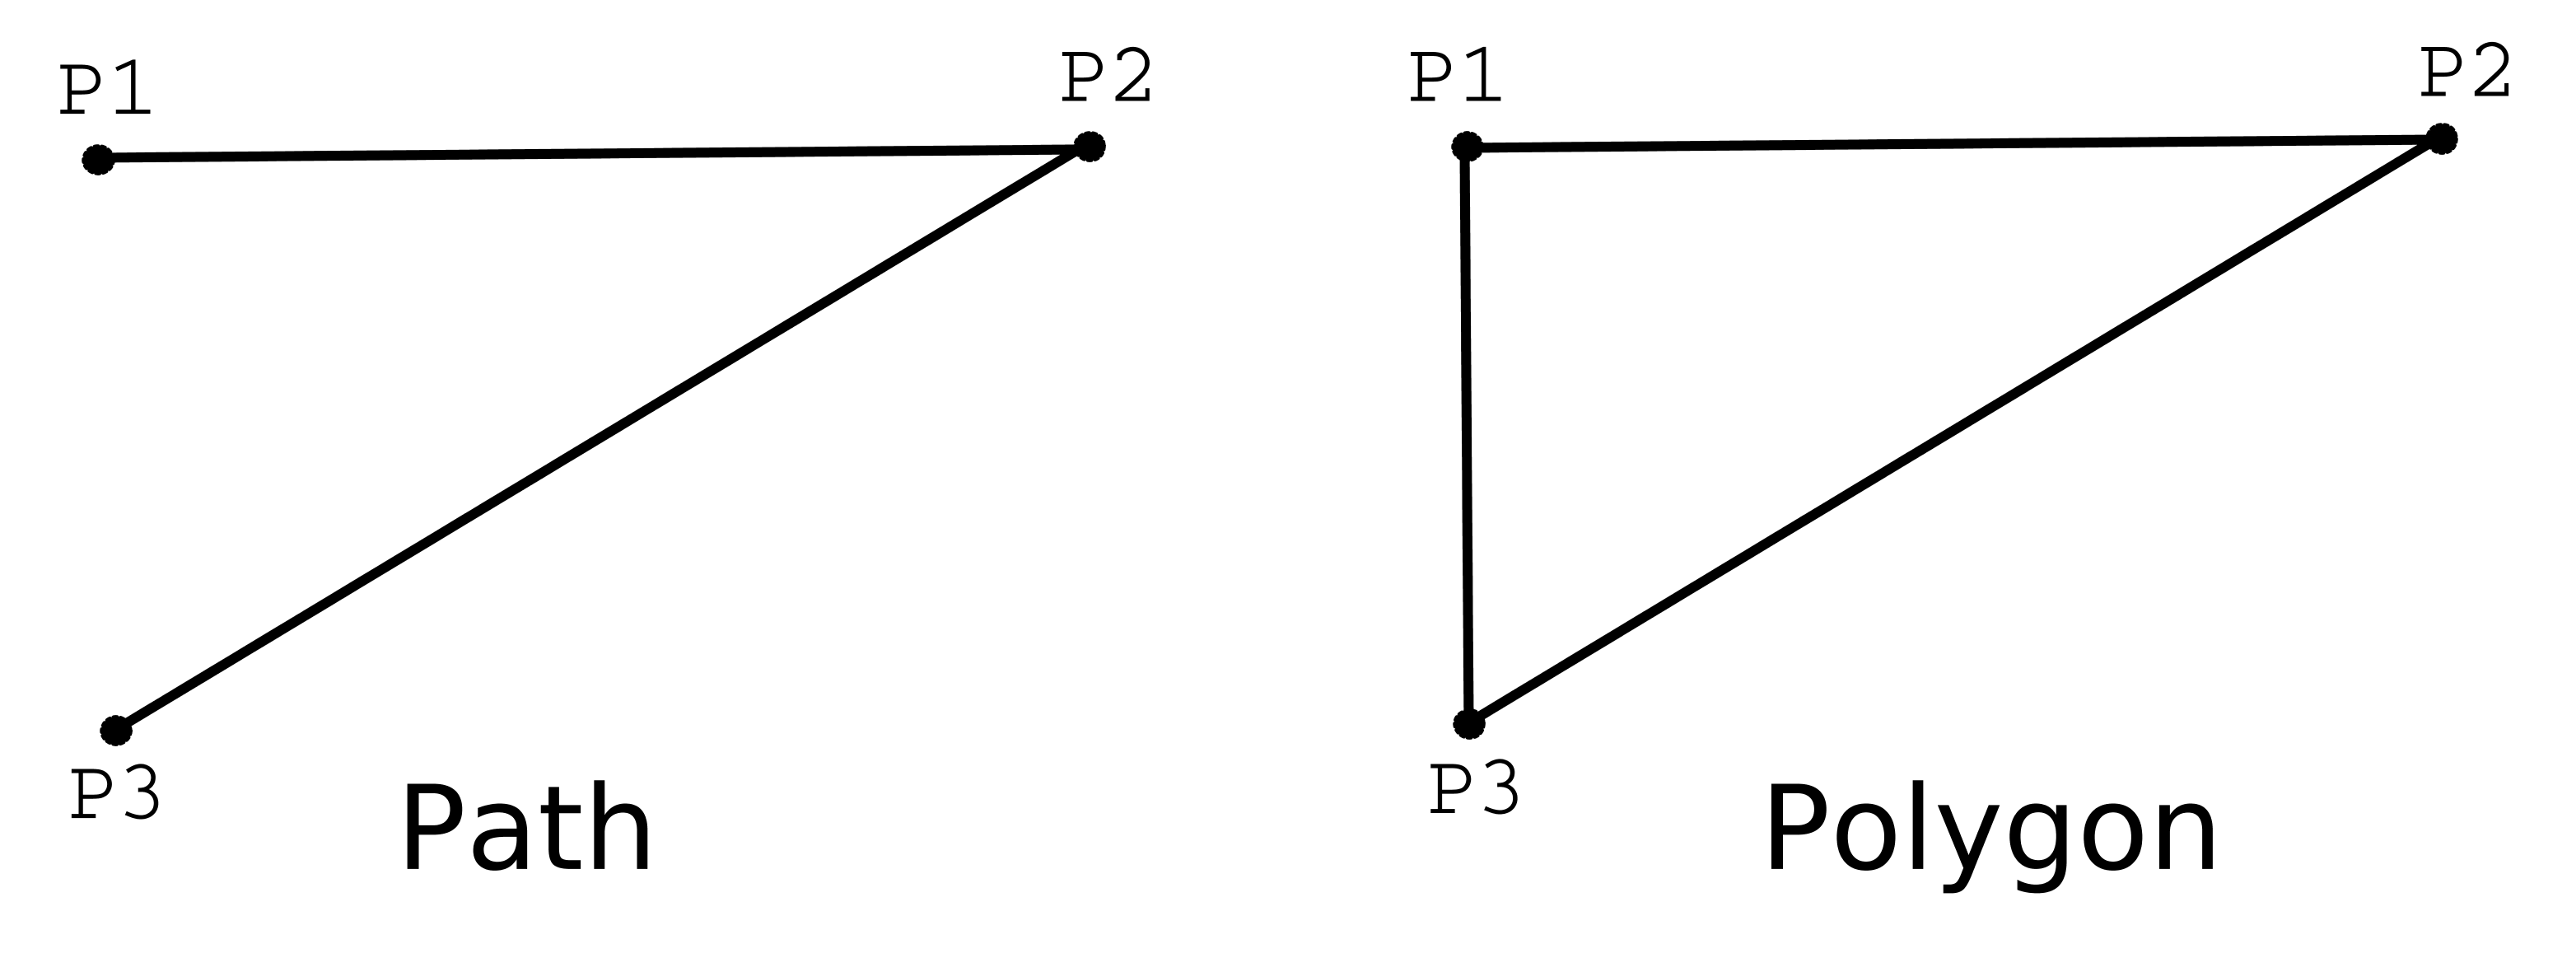
\includegraphics[scale=0.10]{figures/PathVsPolygon}
\end{center}
\caption{Rendering of a Path vs. rendering of a Polygon with the same base points}
\label{PathVsPolygon}
\end{figure}


\subsubsection{Rectangles}
\label{rectangle-class}
% rectangles (with rounded edges)
The \RenderRectangle object was taken from the SVG specification and allows the definition of 
rectangles with or without rounded edges. 

The rectangle has the attributes 
\token{x}, \token{y} and \token{z} to specify its position within the 
bounding box of the enclosing layout object and a \token{width} and 
\token{height} attribute that specifies the width and height of the rectangle, 
either in absolute values or as a percentage of the width and height of the 
enclosing bounding box. The default value for the optional \token{z} attribute 
is $0.0$.

Additionally the rectangle has two optional attributes \token{rx} and
\token{ry} that specify the radius of the corner curvature. If only \token{rx} or \token{ry} 
is specified, the other is presumed to have the same value as the one given. The default value 
for \token{rx} and \token{ry} is $0.0$ which means that the edges are not rounded.
The relative values in rx and ry are in relation to the width and the height of the rectangle respectively.
So a value of $10\%$ for rx means the radius of the corner is $10\%$ of the width of the rectangle. 

\begin{figure}[!ht]
\footnotesize{
\renewcommand{\arraystretch}{1.3}
\begin{tabular}{|lcl|}
\hline
\multicolumn{3}{|c|}{\RenderRectangle inherits from \GraphicalPrimitiveTwoD}\\
\hline
x & : & string \\
y & : & string \\
z & : & string \{use="optional" default="0.0"\}\\
width & : & string \\
height & : & string \\
rx & : & string \{use="optional" default="0.0"\}\\
ry & : & string \{use="optional" default="0.0"\}\\
\hline           
\end{tabular}
}
\renewcommand{\arraystretch}{1.0}

\label{UML:Rectangle}
\end{figure}

\vspace{0.25cm}
{\large
{\bf
example:
}
}

{\footnotesize
\begin{example}
 <g ...>
  <rectangle x="0%" y="0%" width="100%" height="100%" rx="5%" 
             fill="darkred" stroke="#000000" /> 
      ...
</g> 
\end{example}
}

    
\subsubsection{Ellipses}    
\label{ellipse-class}
% ellipses
The definition of an ellipse was also taken directly from SVG. The \texttt{ellipse} element has 
the attributes \token{cx}, \token{cy} and \token{cz} to specify the center 
of the ellipse and \token{rx} and \token{ry} to specify the radius of the 
ellipse along the x-axis and the y-axis respectively. If only \token{rx} or \token{ry} is 
specified, the other is presumed to have the same value. Circles are a special 
case of an ellipse where \token{rx} and \token{ry} are equal. Again \token{cz} is optional and
its default value is $0.0$.

\begin{figure}[!ht]
\footnotesize{
\renewcommand{\arraystretch}{1.3}
\begin{tabular}{|lcl|}
\hline
\multicolumn{3}{|c|}{\RenderEllipse inherits from \GraphicalPrimitiveTwoD}\\
\hline
cx & : & string \\
cy & : & string \\
cz & : & string \{use="optional" default="0.0"\}\\
rx & : & string \\
ry & : & string \{use="optional" default=rx\}\\
\hline           
\end{tabular}
}
\renewcommand{\arraystretch}{1.0}

\label{UML:Ellipse}
\end{figure}

{\large
{\bf
example:
}
}

{\footnotesize
\begin{example}
 <g ...>
  <ellipse cx="50%" cy="50%" rx="30%" fill="#00FF00" stroke="#000000" /> 
      ...
</g> 
\end{example}
}

\subsubsection{Text elements}
\label{text-class}
% text elements
In order to draw text, we use the \token{text} element from SVG with slight 
modifications. Like the \texttt{text} element in SVG, our text element has the 
optional attributes \token{font-family} to specify  which font to use and 
\token{font-size} to specify the size of the font.  
If specified, \token{font-size} must be a positive value. It can be either an absolute
value or a relative value. In the case of a relative value it specifies a percentage of the
height of the corresponding object. Combinations of absolute and relative values as for the 
point objects in other objects are not allowed.

For reasons of simplicity, we limit the display of text to normal text, 
outlined or filled-outlined text are not supported. Also in order to simplify the
text display we think it would be best practice if programs would limit the 
choice of the \token{font-family} attribute to the generic families \token{serif}, \token{sans-serif}
and \token{monospace}. But since those only apply to western languages, it can make
sense to use other values for \token{font-family} in certain cases.

The horizontal alignment of a text element can be specified by the 
\token{text-anchor} attribute. Allowed values are \token{start}, \token{middle} and \token{end}.  Since we feel that this is an important feature, we
have added a corresponding attribute called \token{vtext-anchor} which determines the vertical justification of the
text element. 

The alignment attributes do not have default values because this would disable inheritance. Only the top level group in a style does have default values for the alignment attributes.

Since we have a right handed coordinate system, the positive y axis normally faces downward on the screen if the positive
z-axis goes into the screen. This means that text actually has to be renderer with the top towards lower y-values.

\begin{figure}[!ht]
\begin{center}
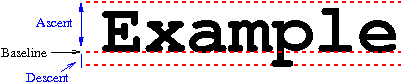
\includegraphics[scale=0.60]{figures/VerticalTextPlacement1}
\end{center}
\caption{example text with marked baseline, ascent and descent}
\label{VerticalTextPlacement1}
\end{figure}


{\color{red} Position of text elements depends on the alignment attributes {\textbf text-anchor} and {\textbf vtext-anchor} as well as the optional offset values which can be given as {\textbf x}, {\textbf y} and {\textbf z}}.
{\color{red} The value given with the {\textbf x} attribute determines where the horizontal text anchor is positioned while the value of the {\textbf y} attribute specifies the position of the vertical text anchor as specified by the {\textbf vtext-anchor} attribute. The {\textbf z} attribute directly specifies the depth value of the text element since there is no alignment attribute for text in the third dimension.}
The default value for all three offset attributes {\textbf x},{\textbf y} and {\textbf z} is $0.0$.

The \texttt{text} element has two more attributes. One is called
\token{font-weight} and specifies whether a font is to be drawn bold. 
Likewise the \token{font-style} attribute determines whether a font is to be
drawn italic or normal and consequently the only allowed values are
\token{italic} and \token{normal}. Both attributes are optional. 

Since the way text is drawn is completely determined by the font specification, text elements should ignore the stroke-width attribute that they inherit from \GraphicalPrimitiveOneD.


\begin{figure}[!ht]
\footnotesize{
\renewcommand{\arraystretch}{1.3}
\begin{tabular}{|lcl|}
\hline
\multicolumn{3}{|c|}{\Text inherits from \GraphicalPrimitiveOneD}\\
\hline
x & : & string \\
y & : & string \\
z & : & string \{use="optional" default="0.0"\}\\
font-family & : & string \{use="optional"\}\\
font-size & : & string \{use="optional"\}\\
font-weight & : & string \{use="optional"\}\\
font-style & : & string \{use="optional"\}\\
text-anchor& : & string \{use="optional"\}\\
vtext-anchor& : & string \{use="optional"\}\\
\hline           
\end{tabular}
}
\renewcommand{\arraystretch}{1.0}

\label{UML:Text}
\end{figure}

\vspace{0.25cm}
{\large
{\bf
example:
}
}

{\footnotesize
\begin{example}
 <g ...>
  <text x="50%" y="50%" text-anchor="middle" stroke="#FF0000"
        font-family="serif" font-size="20.0" >This is a Text</text> 
     ...
</g> 
\end{example}
}


\subsubsection{Bitmaps}
\label{image-class}
To include bitmaps into a graphical representation we use the \Image element 
from SVG. The \Image element in SVG can also be used to include complete SVG 
vector images which we explicitly exclude in this version of the proposal 
since we think it would be too complex. If the need for the inclusion of SVG 
drawings arises, it is only a matter of rephrasing this specification.

In addition to the optional id attribute, the \Image element has six attributes. The \token{x}, \token{y} and 
\token{z} attributes specify the position of the image within the bounding box 
and the \token{width} and \token{height} attributes specify its width and 
height. The \token{z} attribute is optional and its default value is $0.0$. 
The actual image data is not embedded in the render information, but the \Image 
element has an attribute called \token{href} that references an 
external JPEG or PNG file. To simplify things, the reference has to be an absolute or relative path to a local file.
Non-local image resources (e.g. from the net) are currently not supported.
If the referenced image is larger then the given 
width and height, it has to be scaled to the given dimensions.
If the reference resource can not be found, it is up to the application if nothing is drawn or some place holder is displayed.
Preferably the user would get some kind of notification about the missing resource.

\begin{figure}[!ht]
\footnotesize{
\renewcommand{\arraystretch}{1.3}
\begin{tabular}{|lcl|}
\hline
\multicolumn{3}{|c|}{\Image inherits from {\TransformationTwoD}}\\
\hline
id & : & SId \{use="optional"\}\\
x & : & string \\
y & : & string \\
z & : & string \{use="optional" default="0.0"\}\\
width & : & string \\
height & : & string \\
href & : & string \\
\hline           
\end{tabular}
}
\renewcommand{\arraystretch}{1.0}

\label{UML:Image}
\end{figure}


\vspace{0.25cm}
{\large
  {\bf
example:
}
}
{
\footnotesize
\begin{example}
 <g ...>
  <image x="10%" y="10%" width="80" height="100" href="Glucose.png" /> 
      ...
</g> 
\end{example}
}


\subsubsection{Grouping}
\label{group-class}
Like in SVG, several graphical primitives can be grouped inside a \texttt{g} 
element to generate more complex render information.


\begin{figure}[!ht]
\footnotesize{
\renewcommand{\arraystretch}{1.3}
\begin{tabular}{|lcl|}
\hline
\multicolumn{3}{|c|}{\Group inherits from \GraphicalPrimitiveTwoD}\\
\hline
font-family & : & string \{use="optional"\}\\
font-size & : & string \{use="optional"\}\\
font-weight & : & string \{use="optional"\}\\
font-style & : & string \{use="optional"\}\\
text-anchor& : & string \{use="optional"\}\\
vtext-anchor& : & string \{use="optional"\}\\
startHead & : & SId \{use="optional"\}\\
endHead & : & SId \{use="optional"\}\\
\hline           
\end{tabular}
}
\renewcommand{\arraystretch}{1.0}

\label{UML:Group}
\end{figure}



\textbf{stroke}, 
\textbf{stroke-width}, \textbf{stroke-dash\-arrays}, \textbf{transform}, 
\textbf{fill},{\textbf{fill-rule}}, \textbf{font-family}, \textbf{font-size}, \textbf{font-weight}, 
\textbf{font-style} and \textbf{text-anchor} attributes can be applied to 
groups. If any of those attributes is specified for a \Group object, it 
specifies the corresponding attribute for all graphical primitives and groups 
defined within this group. If a graphical primitive or a group redefines one or 
more of those attributes, the newly defined values take effect. 
The outermost group in a style always has default values for the attributes, all other embedded elements don't
have default values for their attributes. This way it is easy to distinguish between an attribute that
has really been set and one that has not been set.
The default values for the outermost \texttt{group} element are listed in table \ref{attribute_defaults}. 

\vspace{0.5cm}
\begin{table}[h]
\begin{center}
\begin{tabular}{|c|c|}\hline
\textbf{attribute} & \textbf{default value} \\ \hline\hline
stroke & none \\ \hline
stroke-width & 0.0 \\ \hline
stroke-dasharrays & \textit{empty list} \\ \hline
transform &  1.0, 0.0, 0.0, 0.0, 1.0, 0.0 \\ \hline
fill & \textbf{none}\\ \hline
fill-rule & string \{use="optional" default="nonzero"\}\\ \hline
font-family & sans-serif \\ \hline
font-size & 0 \\ \hline
font-weight & normal \\ \hline
font-style & normal \\ \hline
text-anchor & start\\ \hline
vtext-anchor & top\\ \hline
startHead & \textbf{none} \\ \hline
endHead & \textbf{none} \\ \hline
\end{tabular}
\end{center}
\caption{Attribute default values.}
\label{attribute_defaults}
\end{table}
\vspace{0.5cm}

It might seem a little unusual that the default values for \textbf{stroke-width} and
\textbf{font-size} are set to 0. The reason for this is that a style that only contains
an empty \texttt{group} is meant to define that the element the style applies to is not
to be rendered. Since the render information for curves in
\SpeciesReferenceGlyph and \ReactionGlyph objects as well as the render information for
\textbf{TextGlyph} objects is defined via attributes from the outermost \texttt{group} element of a
style (see below), the \texttt{group} element would explicitly have to define the \textbf{stroke-width} or the
\textbf{font-size} to be 0 which would be inconsistent with the implied meaning of an
empty group.
The outermost \texttt{group} element can also contain information about arrow heads to be used on curves 
specified in the layout. This information is given via the \textbf{startHead} and \textbf{endHead}
attributes just like for \texttt{curve} elements. These attributes only apply to \RenderCurve objects from the layout, not
to \textbf{RenderCurve} objects within the group. Since those two attributes only make sense on the outermost group of a style,
they are to be ignored on all other groups. The default value for those attributes is \texttt{none} which means that 
no line ending is to be drawn. 


Each \texttt{group} element also has an \textbf{id} attribute through which it can be identified. 
In addition to those attributes a \Group object can contain 0 or more child
elements that form the render information. These child elements have to be elements derived from \TransformationTwoD,
so right now this would be {\Image}s or everything derived from \GraphicalPrimitiveOneD,
e.g. \texttt{rectangles}, \texttt{ellipses}, \texttt{curves}, \texttt{polygons}, \texttt{text} elements
or \texttt{groups}.

{\large
{\bf
example:
}
}

{\footnotesize
\begin{example}
 <g stroke="#000000" font-family="serif" >
   <rectangle x="0%" y="0%" width="100%" height="100%" 
              fill="blueLinearGradient"	 />
   <text x="50%" y="50%" font-size="80%" text-anchor="middle" 
         stroke="#FF0000" />
</g> 
\end{example}
}

\subsection{Line endings}
\label{lineending-class}
In many graphs the relations between nodes are depicted by lines and often the 
type of relation is encoded in the line ending. For this reason, the render
extension provides ways to specify a set of arbitrary line endings and means to
apply those to path objects.
The individual line endings are defined in an element called
\texttt{listOfLineEndings} which comes right before the \texttt{listOf\-Styles}.

The individual line endings are defined as \Group objects just like styles. 
Therefore, 
arbitrarily complex line endings can be defined. Each line ending is
encapsulated in an element called \texttt{lineEnding} and contains two
sub elements. 

The first element is called \texttt{boundingBox} and it specifies the
viewport that is used to draw the line ending. Just like the bounding boxes of
the layout extension, this bounding box contains a \texttt{position} and a
\texttt{dimensions} sub element. The \texttt{dimensions} element  
specifies the size of the view port for the line ending along each of the axes. 
The \texttt{position} element specifies the offset from the end of the curve that the line ending is applied to.
A position of $(0.0, 0.0, 0.0)$ means that the origin of the line endings bounding box is mapped directly to
the end of the curve. For a description on how the mapping is calculated in all other cases see the section called "Mapping line endings to curves".


The second sub-element is a \texttt{group} element that holds the render
information for the line ending. 

The two attributes of the \texttt{lineEnding}
element are the \textbf{id} attribute which is used to specify a unique id for
the line ending by which it can be referenced and an attribute called \textbf{enable\-Rotational\-Mapping}.
The \textbf{enable\-Rotational\-Mapping} attribute specifies whether a line ending
will be rotated depending on the slope of the line it is applied to or if it is
drawn just the way it was specified. The default value for the attribute is
\texttt{true} which means that the line ending is rotated depending on the
slope of the line. A more detailed description of this mapping is given in figure \ref{EnableRotationalMapping}.

In order to declare that a certain line ending is to be used on a path object,
the \texttt{curve} element has two attributes called \textbf{startHead} and
\textbf{endHead} which hold the id of a line ending definition for the start and 
for the end of the path respectively.

The top level group in a line ending differs from top level groups in normal graphical elements in one respect. The top level group of a line ending inherits all attributes from the line it is applied to save for the attributes for the line endings themselves. This way a style sheet can define one line ending which can be applied to lines of different colors and it inherits the color from the line.
If the group also inherited the attributes for the line endings and it contained a \texttt{curve} element itself, we would have generated an endless loop.

\begin{figure}[!ht]
\footnotesize{
\renewcommand{\arraystretch}{1.3}
\begin{tabular}{|lcl|}
\hline
\multicolumn{3}{|c|}{\LineEnding inherits from \GraphicalPrimitiveTwoD}\\
\hline
enableRotationalMapping & : & boolean {default=true} \\
boundingBox & : & BoundingBox \\
g & : & Group \\
\hline           
\end{tabular}
}
\renewcommand{\arraystretch}{1.0}

\label{UML:LineEnding}
\end{figure}

\vspace{0.25cm}
{\large
  {\bf
example:
}
}
{
\footnotesize
\begin{example}
<lineEnding id="SimpleArrowHead">
 <boundingBox>
   <position x="-10.0" y="-4.0" />
   <dimensions width="12.0" height="8.0"/>
 </boundingBox>
 <g>
   <polygon>
     <curve>
       <listOfCurveSegments>
         <curveSegment xsi:type="LineSegment">
           <start x="100%" y="50%" />
           <end x="0%" y="100%" />
         </curveSegment>
         <curveSegment xsi:type="LineSegment">
           <start x="0%" y="100%" />
           <end x="0%" y="0%" />
         </curveSegment>
       </listOfCurveSegments>
     </curve>
   </polygon>
 </g>
</lineEnding>  
\end{example}
}

\begin{figure}[!ht]
\begin{center}
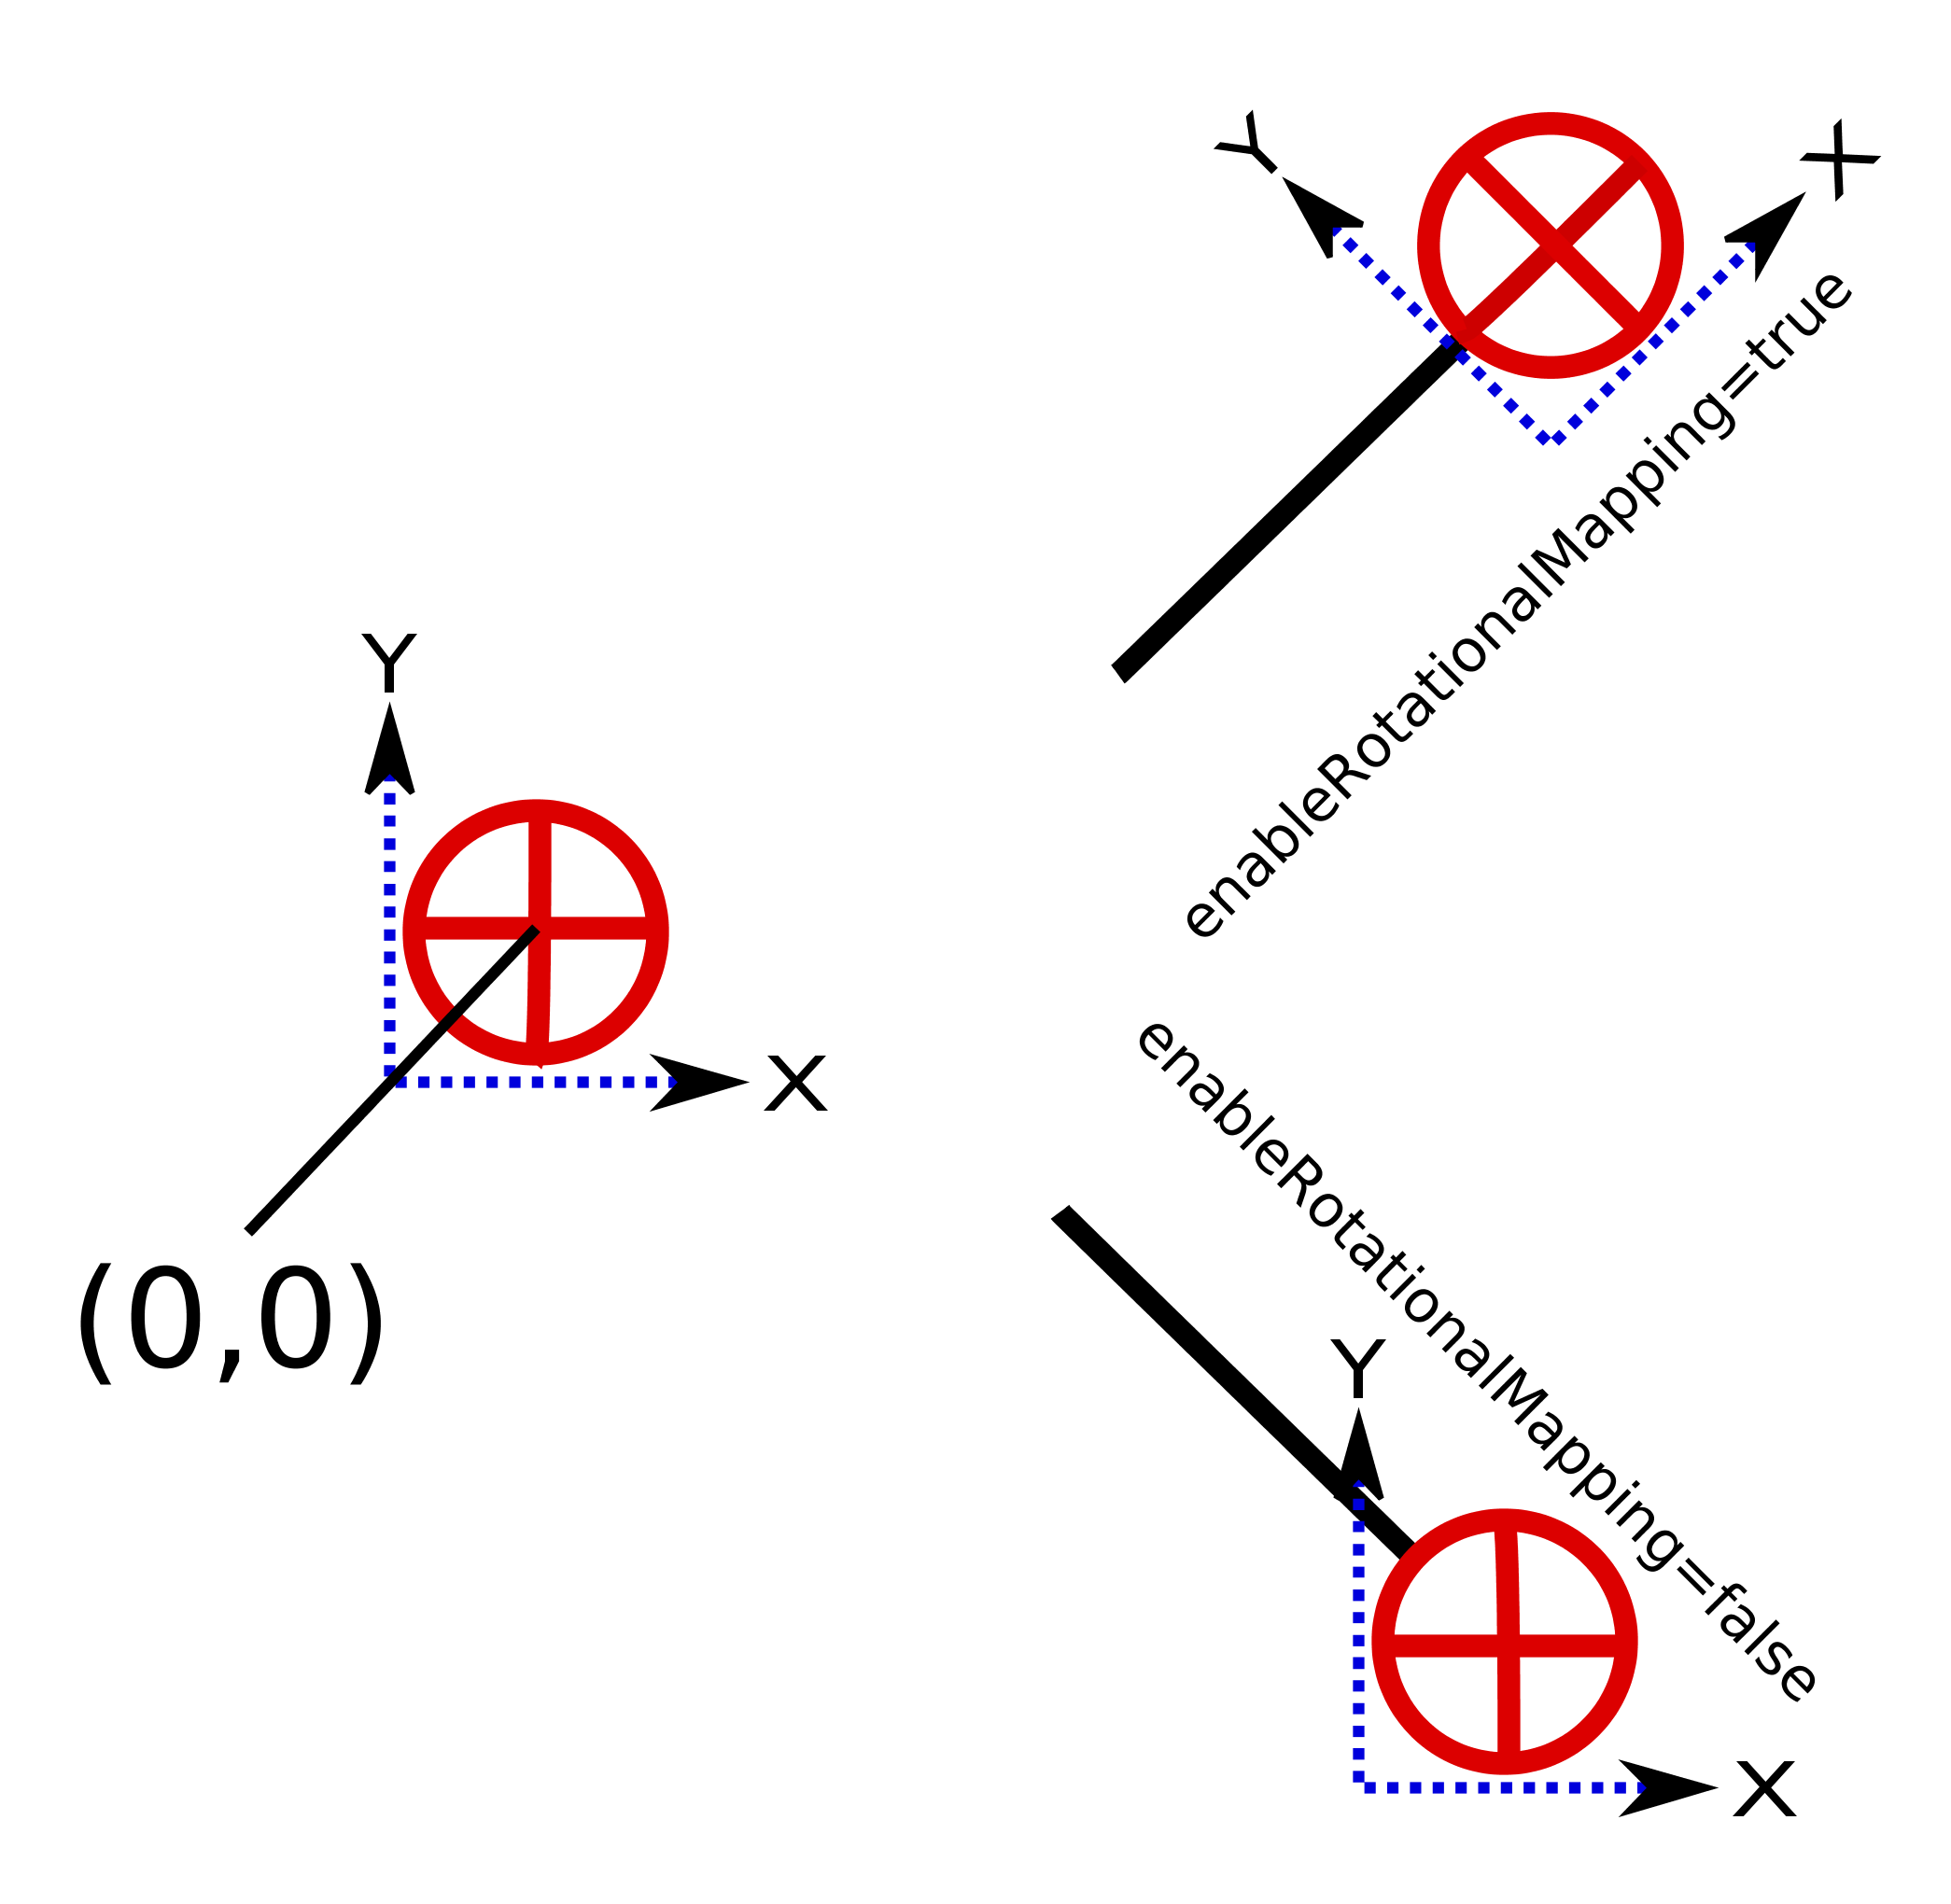
\includegraphics[scale=0.15]{figures/EnableRotationalMapping.png}
\end{center}
\caption{example of a line ending with and without rotation mapping enabled}
\label{EnableRotationalMapping}
\end{figure}


\subsubsection{Mapping line endings to curves}

In order to apply a line ending which is defined using only 2D coordinates onto a line which
has been defined using 3D coordinates, we need to define a kind of mapping.
The first definition we make is that the origin of the line ending view port is
mapped to the end of the line to which the line ending is applied.
If the \token{enable\-Rotational\-Mapping} attribute is set to \val{false}, the
line endings coordinate system is the same as the global coordinate system used to draw the layout,
only the origin is moved to that end of the line the line ending is applied to. If
the \token{enable\-Rotational\-Mapping} attribute is set to \val{true}, which is
the default, we define that the x,y-plane of the line endings view port is mapped to the
plane that results from taking the unit vector of the slope of the line and the unit
vector that results from ortho-normalizing the slope vector and a second vector
that has no component along the z axis. If the slope of the line has a positive component along the x axis,
the ortho-normalized vector also has to have a positive component along the y axis. In order to retain the
right handed coordinate system, the z axis of the line endings coordinate system is perpendicular to the plane created by the other two vectors and has a positive component along the global coordinate systems z-axis.
Likewise if the slope has a negative component along the global coordinate systems x axis, the y component of the
ortho-normalized second vector has a negative component along the y axis of the global coordinate system and to 
retain the right handed coordinate system, the third vector which is perpendicular to the plane made by the slope
and its ortho-normalized vector, has a positive component along the global coordinate systems z axis. 

If the slope of the line points directly along the positive z axis of the global coordinate system, the 
line endings coordinate system is mapped to the line ending by a -90 rotation around the y axis of the 
line endings coordinate system and a translation of the origin of the line endings coordinate system to 
the end of the line. If the slope points directly down the negative z axis, the line endings coordinate 
system has to be rotated by +90 around its y axis before translation to the position of the curves end.   

This may all sound very complicated, but in the end, the calculations to be done are not difficult and straight forward. 

The mathematical description of the mapping and an example are given in Appendix A.


\subsection{Style resolution}
To resolve which style applies to a certain object, one 
should follow the rule that more specific style definitions take precedence 
over less specific ones and that if there are several styles with the same 
specificity, the first one encountered in the file is to be used. In essence,
this means that a program first has to search the local render information for 
a style that references the id of the object. If none is found, it searches for 
a style that mentions the role of the object. If it has one, see next section. 
If it does not find one, it searches for a style for the type of the object. 

If a render information references another render information object via its 
\token{reference\-Render\-Information} attribute, the program has to go through 
that one as well to see if a more specific render information is present there. 
If the chain of referenced \RenderInformation objects has been searched and no 
style has been found that fits, it is up to the program how the object is 
rendered. 

If several type based styles are found 
that would fit, a style that applies to only one type takes precedence over a 
style that applies to several types.

If a program explicitly wants to define render information that 
states that some objects are not to be rendered at all, it has to define a 
style that does nothing, i.e. has no render information but applies to the 
objects that should not be rendered. 


\subsection{Role resolution}
This render extension explicitly provides means to write render information
that renders layout objects based on certain roles those render objects or their
corresponding model objects have. So far SBML models or layouts do not contain
such role information or only for a limited number of objects if one would
consider the role attribute of \SpeciesReferenceGlyph objects to fall into this category.
Although there is currently no means to specify these roles, there are already
initiatives underway that try to complement SBML files with more biological
information based on ontologies. One of these initiatives, the sboTerms, is
about to be included into SBML Level 2 Version 2. This ontology or a similar
one could provide this role information for layout objects in the future.   

For the time being, we define an additional attribute called \token{objectRole} for all 
layout objects derived from \GraphicalObject including \GraphicalObject itself.
The attribute specifies a user defined role string. render information including the same role string in its
\token{roleList} attribute applies to the object. This is only true if no more specific render information
takes precedence (see "Style resolution").
 
A specific style can reference one or more roles to which it applies. When a program tries to determine which style applies to a 
specific object it might have to determine the role of the object layout first. If the 
layout object itself has a role, this will be taken, otherwise if the layout object 
is associated with an object in the model, the program should get the role from 
the associated object. If none of them has a role, no role based style can be 
applied to the object.

\subsection{Style information for reaction glyphs and species reference glyphs}

When defining a style for a \ReactionGlyph or \SpeciesReferenceGlyph object, one 
has to distinguish between layout objects that only specify a bounding box for the 
object and those that specify a curve. In the case of a bounding box, you want to 
define complete render information, whereas in the case of a curve, you only 
want to set certain attributes that determine certain aspects of how the 
curve should be drawn, e.g. its color. To resolve this conflict, the style for such an 
object has to define render information for both cases. The render information 
for the case of a bounding box is specified just like render information for 
any other object within a group. Render information for the case of a curve is 
defined by the appropriate attributes that are in effect in the outermost \Group 
object itself. Those attributes include \token{stroke}, \token{stroke-width} 
and \token{stroke-dasharray}. Additionally \token{startHead} and \token{endHead} can be 
specified to define line endings for layout curve objects. If the group does not define 
one or more of these attributes, the default value is used (see section "Grouping").

\begin{figure}[!ht]
\begin{center}
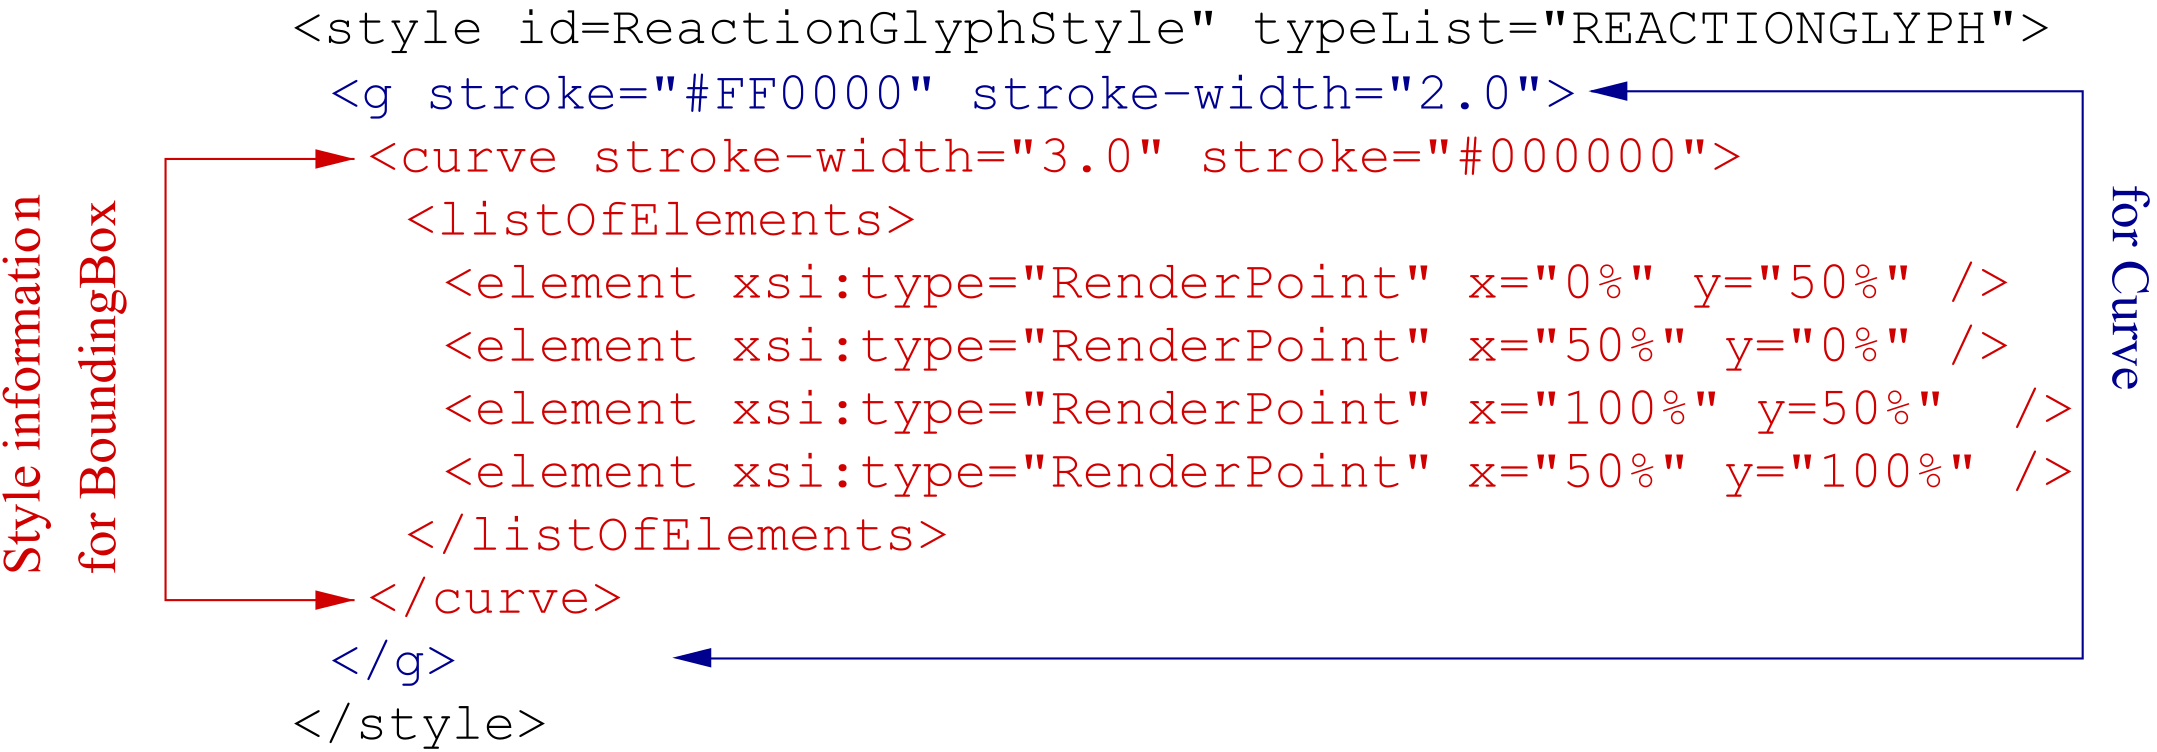
\includegraphics[scale=0.25]{figures/CurveAndBBStyle}
\end{center}
\caption{style with render information for objects with curve or bounding box}
\label{CurveAndBBStyle}
\end{figure}

\subsection{Style information for text glyphs}
Just as in the case of curves in {\ReactionGlyph}s and {\SpeciesReferenceGlyph}s,
{\TextGlyph}s can be considered render information which is located
in the layout. A \TextGlyph specifies the text to be rendered,
it therefore does not need additional render information in the form of
a \texttt{text} element. On the other hand, it needs render information in the form of font properties.
Just as for the \RenderCurve
object for {\ReactionGlyph}s and {\SpeciesReferenceGlyph}s, this render information is
taken from the font related attributes of the outermost group element of the
style that is used to render a \TextGlyph. Any additional information within the
group is ignored. If the group does not specify any of the \token{font-family},
\token{font-size}, \token{font-weight}, \token{font-style}, 
\token{text-anchor} or \token{vtext-anchor} attributes, the default values are to be used.


\section{Appendix A}

The mapping of arrow heads to line endings involves some transformations which we would like to illustrate with two examples.
The first example as depicted in Figure \ref{fig:2ArrowHeadMapping} defines a straight line and a line ending which is to be applied
to the end of the line. The line ending specifies a bounding box with a size of 4x4 and a position of $P(-2,-2)$. 
The origin of the line ending is at $o(0.0,0.0,0.0)$ and the bounding box extends along the positive x- and y-axes.
The position of the bounding box is the offset by which the origin of the bounding box has to be translated from the endpoint of the curve.

\begin{figure}[!ht]
\begin{center}
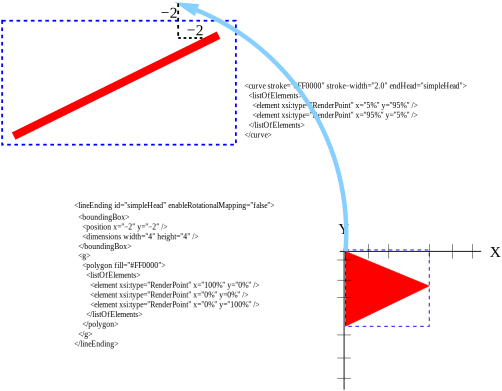
\includegraphics[scale=0.25]{figures/ArrowHeadMapping2}
\end{center}
\caption{Curve with arrow head and no rotational mapping} \label{fig:2ArrowHeadMapping}
\end{figure}

Since the arrow head in the first example explicitly disables rotation mapping by specifying \textbf{enableRotationalMapping=false}
in the definition of the line ending, the process of mapping the arrow head to the line is simply a matter of moving the origin of 
the line endings coordinate system to the end point of the line $E(ex,ey)$ plus the offset that is specified as the position $P(px,py,pz)$ of the line endings bounding box $F=E+P=(ex+px,ey+py,ez+pz)$. In our example the origin of the line endings coordinate system has to be moved 2 units up and two to the left of the and of the curve that the line ending is applied to.

The result of this operation is depicted in Figure \ref{fig:3ArrowHeadMapping}.

\begin{figure}[!ht]
\begin{center}
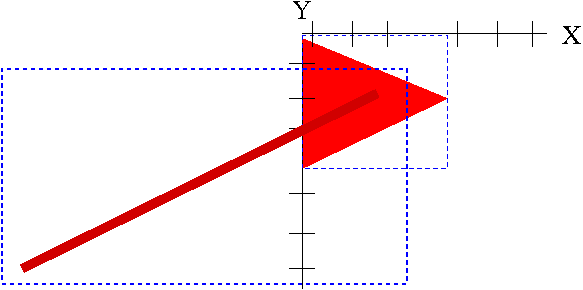
\includegraphics[scale=0.25]{figures/ArrowHeadMapping3}
\end{center}
\caption{Curve with mapped arrow head and no rotational mapping} \label{fig:3ArrowHeadMapping}
\end{figure}

The second example is very similar to the first example, only now, the rotational mapping for the arrow head is enabled.
This means that we now have to execute two steps in order to map the arrow head to the line ending.

First we need to rotate the arrow head so that the x-axis of the arrow heads coordiante system is aligned with the slope $s=\frac{dy}{dx}$ of the curve.

\begin{figure}[!ht]
\begin{center}
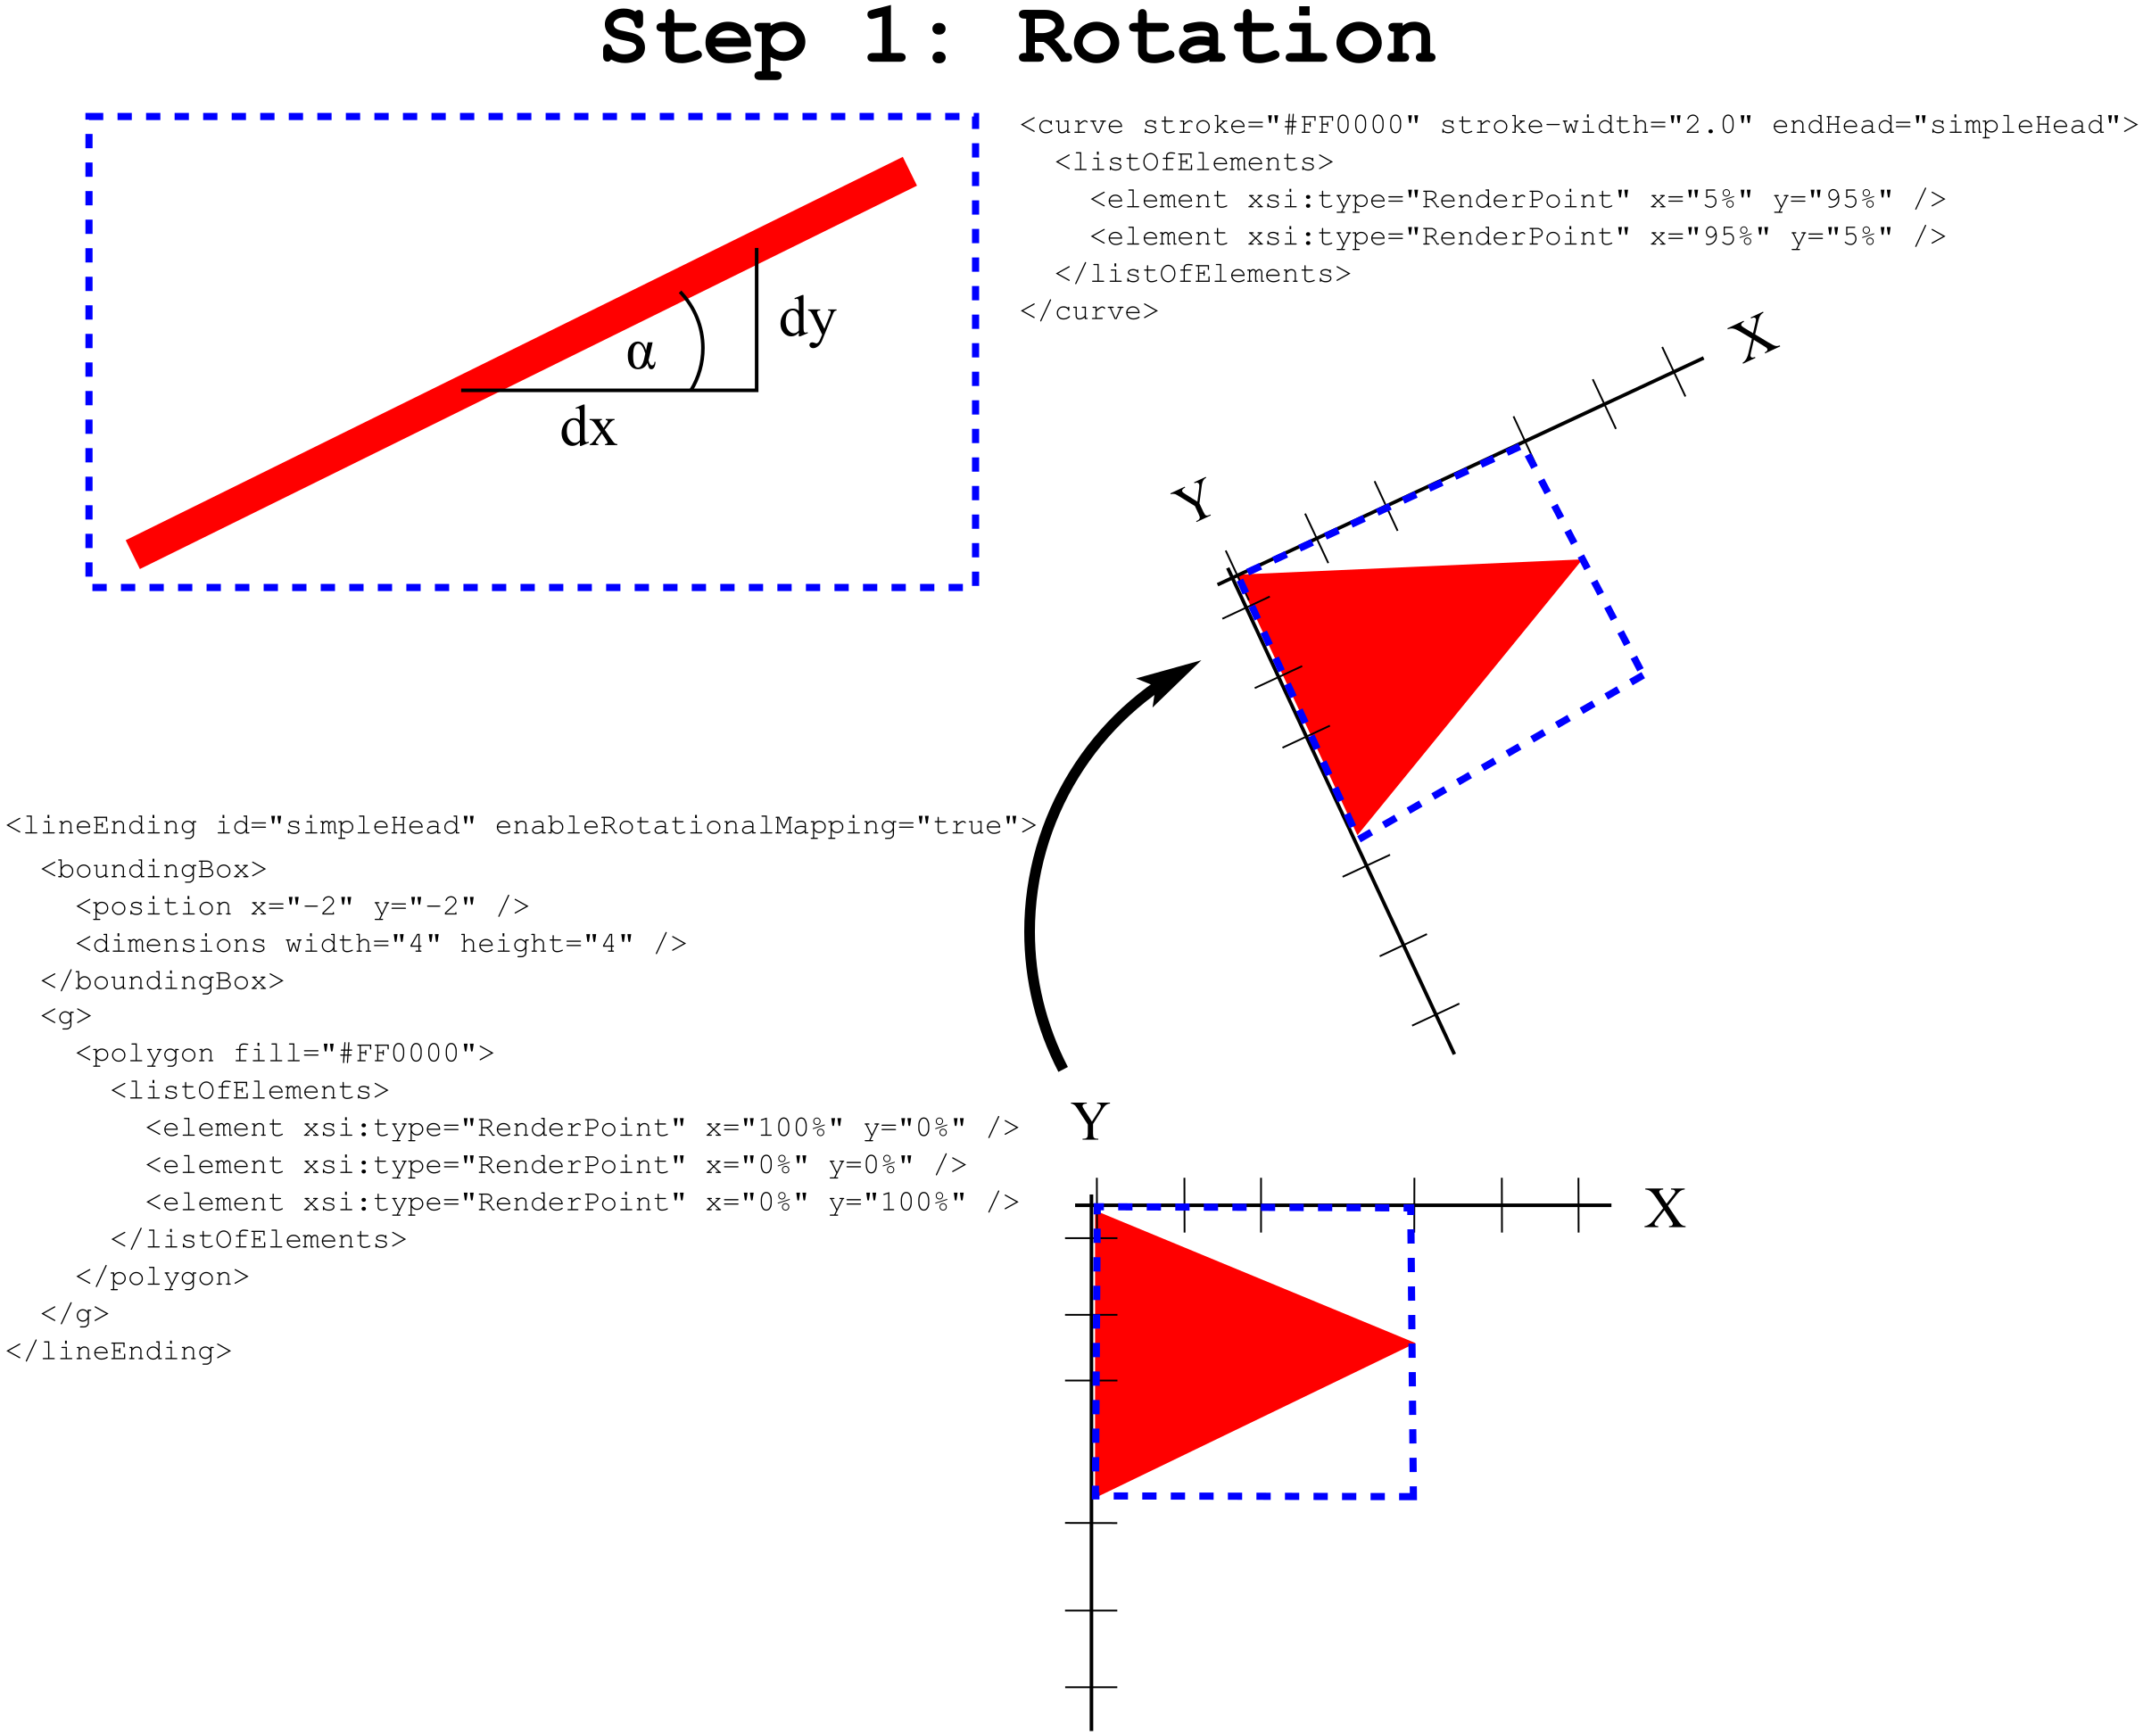
\includegraphics[scale=0.25]{figures/ArrowHeadMapping6}
\end{center}
\caption{Step 1: Rotation}
\label{ArrowHeadMapping6}
\end{figure}

The rotation of the arrow head involves the following steps:

\begin{enumerate}
\item{calculate the normalized direction vector of the slope:\\
We first need to find the two points that determine the slope at the end of the line. One point is always the endpoint of 
the line ($E(ex,ey,ez)$). The second point depends on whether the last element of the line is a straight line or if it is
a bezier element. If it is a bezier element, the second point is the second base point of the bezier element, if it is a 
straight line, it is either the preceding point or the endpoint of the preceding bezier element. We call this second
point $S(sy,dy,sz)$.\\ The direction vector can be calculated as $v(vx,vy,vz)=(ex-sy.ey-sy,ez-sz)$. To normalize the vector
we have to calculate the length $l=\sqrt{vx^2+vy^2+vz^2}$ of the direction vector and divide all elements of $v$ by this
length. $v_n(v_{n}x,v_{n}y,v_{n}z)=(vx/l,vy/l,vz/l)$}

\item{calculate the normalized vector that is
\begin{enumerate}
\item{orthogonal to the direction vector of the line}
\item{located in the plane x- and y-axis}
\end{enumerate}
If the direction vector is parallel to the y-axis $(vx=0.0)$, the orthogonal vector $w$ is parallel to the x-axis ($w(vy,0,0)$).
For all other cases $w$ is $w(wx,wy,wz)=(-v_{n}y*v_{n}x,1-v_{n}y^2,-v_{n}y*v_{n}z)$.\\ Again we have to normalize this
vector by dividing through its length $n=\sqrt{wx^2+wy^2+wz^2}$, which results in the normlized vector\\
$w_n(w_{n}x,w_{n}y,w_{n}z)=(wx/n,wy/n,wz/n)$.
}
\item{create the transformation matrix that converts the original coordinate system into the coordinate system
that is made up of the two calculated vectors:\\
\vspace*{0.3cm}
The transformation matrix that results from the two normalized vector that we calculated in the steps above
is $m=\left(\begin{array}{cccc} v_{n}x & w_{n}x & 0.0 & 0.0\\ v_{n}y & w_{n}y & 0.0 & 0.0\\ v_{n}z & w_{n}z & 0.0 & 1.0 \end{array}\right)$}
\end{enumerate}


The second step moves the origin of the arrow heads coordinate system to the endpoint of the line, which is exactly the same as we did in the first example.

\begin{figure}[!ht]
\begin{center}
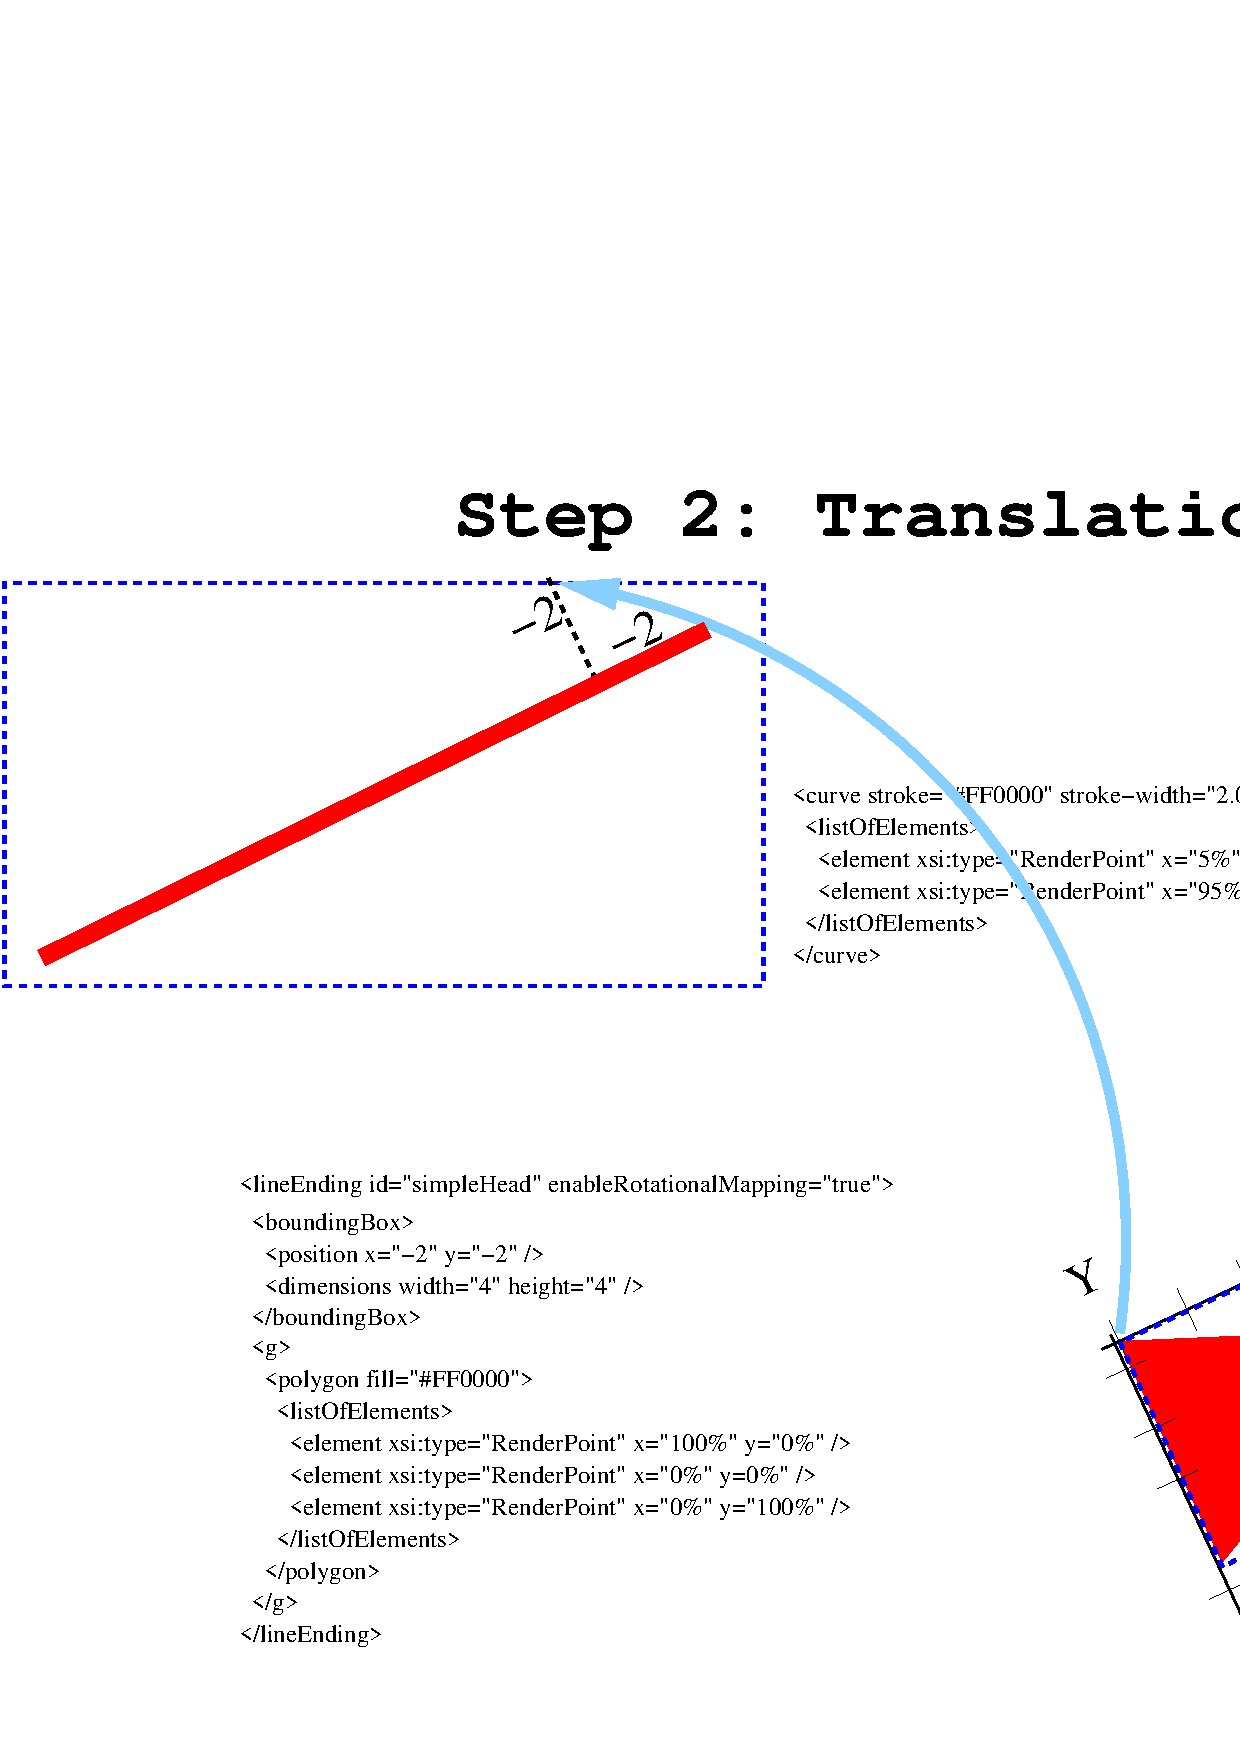
\includegraphics[scale=0.25]{figures/ArrowHeadMapping4}
\end{center}
\caption{Step 2: Translation}
\label{ArrowHeadMapping4}
\end{figure}

\begin{figure}[!ht]
\begin{center}
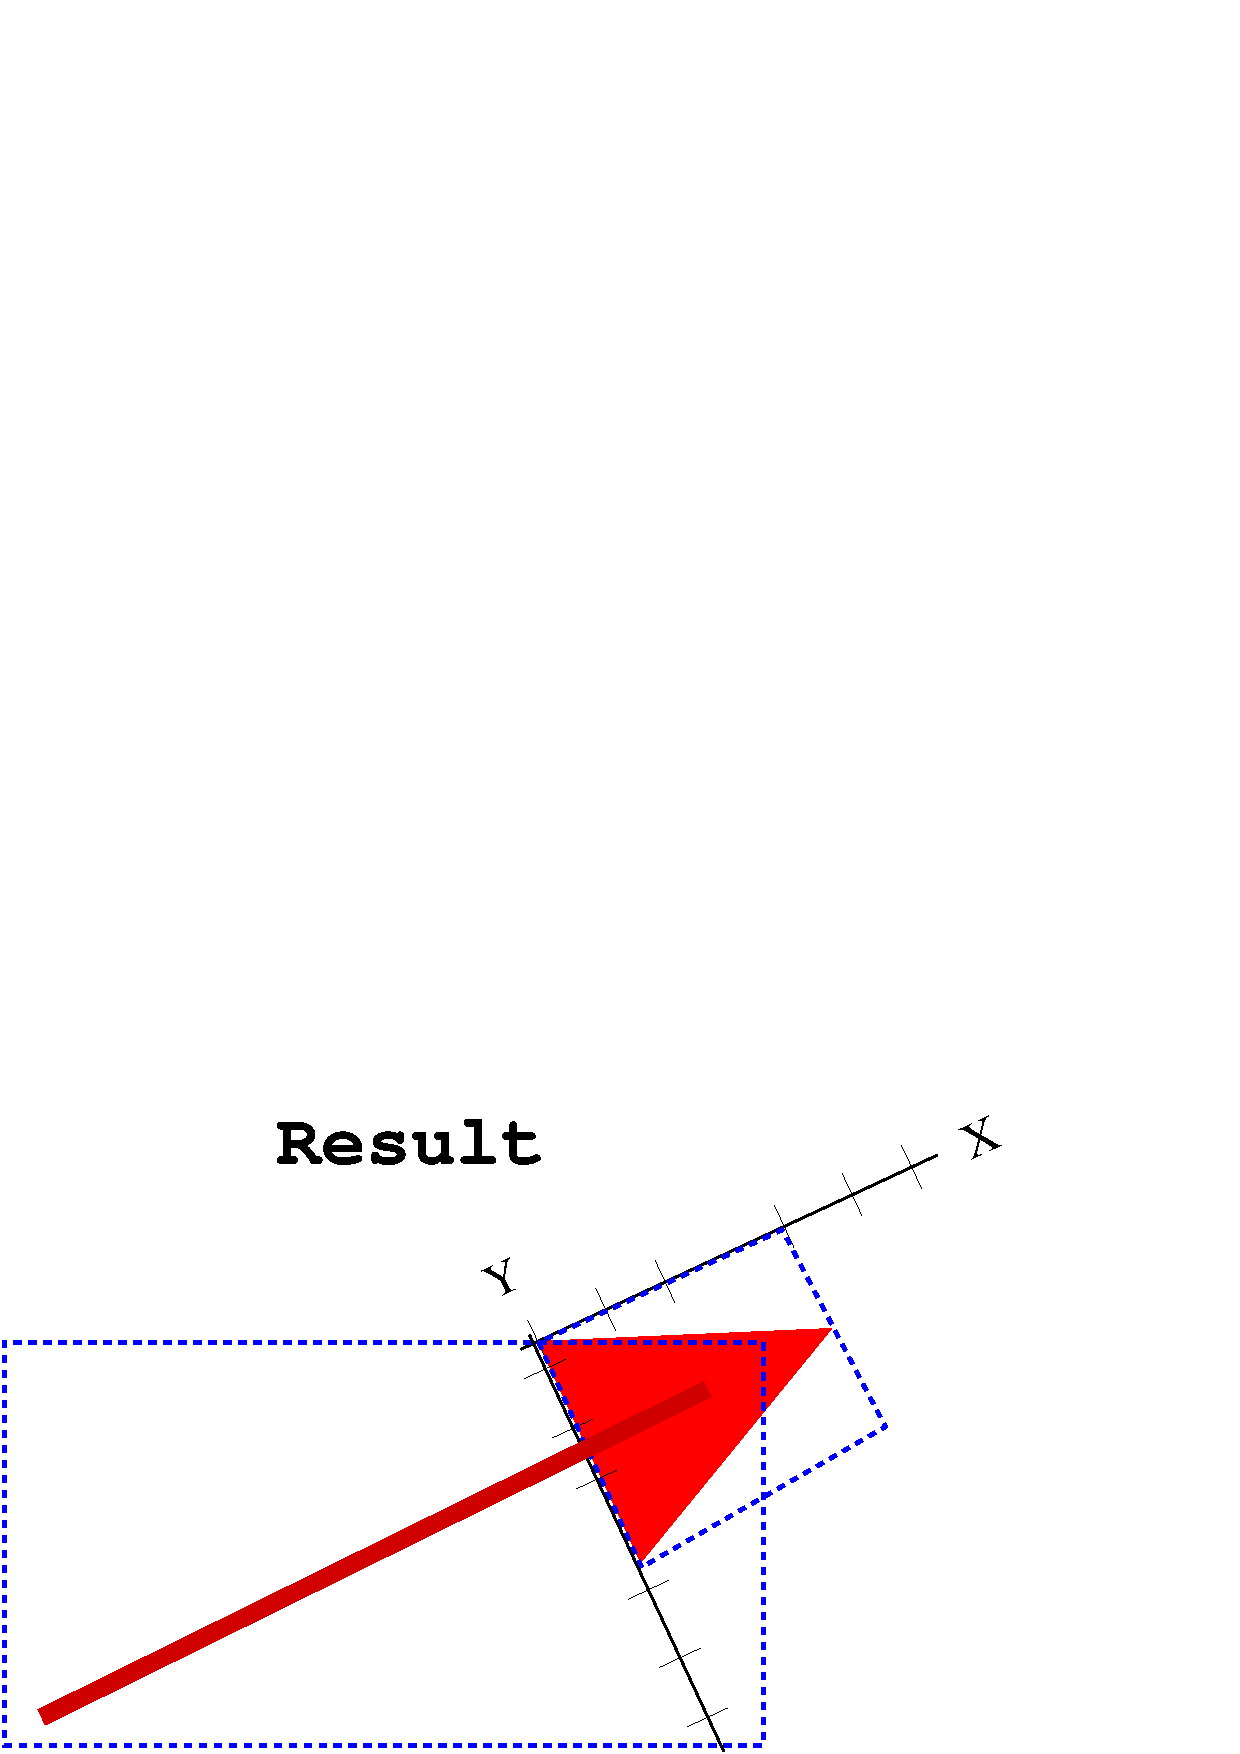
\includegraphics[scale=0.25]{figures/ArrowHeadMapping5}
\end{center}
\caption{Curve with mapped arrow head and rotational mapping}
\label{ArrowHeadMapping5}
\end{figure}

Mapping of an arrow head to the beginning of a curve is exactly the same as for the end of a curve, only the
direction of the line has to be reversed and in case of a cubic bezier, one has to use the first base point rather than the second base point. 

The following four figures are generated from this example using the xslt style sheet implementation with xsltproc.
The SVG images were then rendered with the Chrome Browser from Google.

\begin{figure}[!ht]
\begin{center}
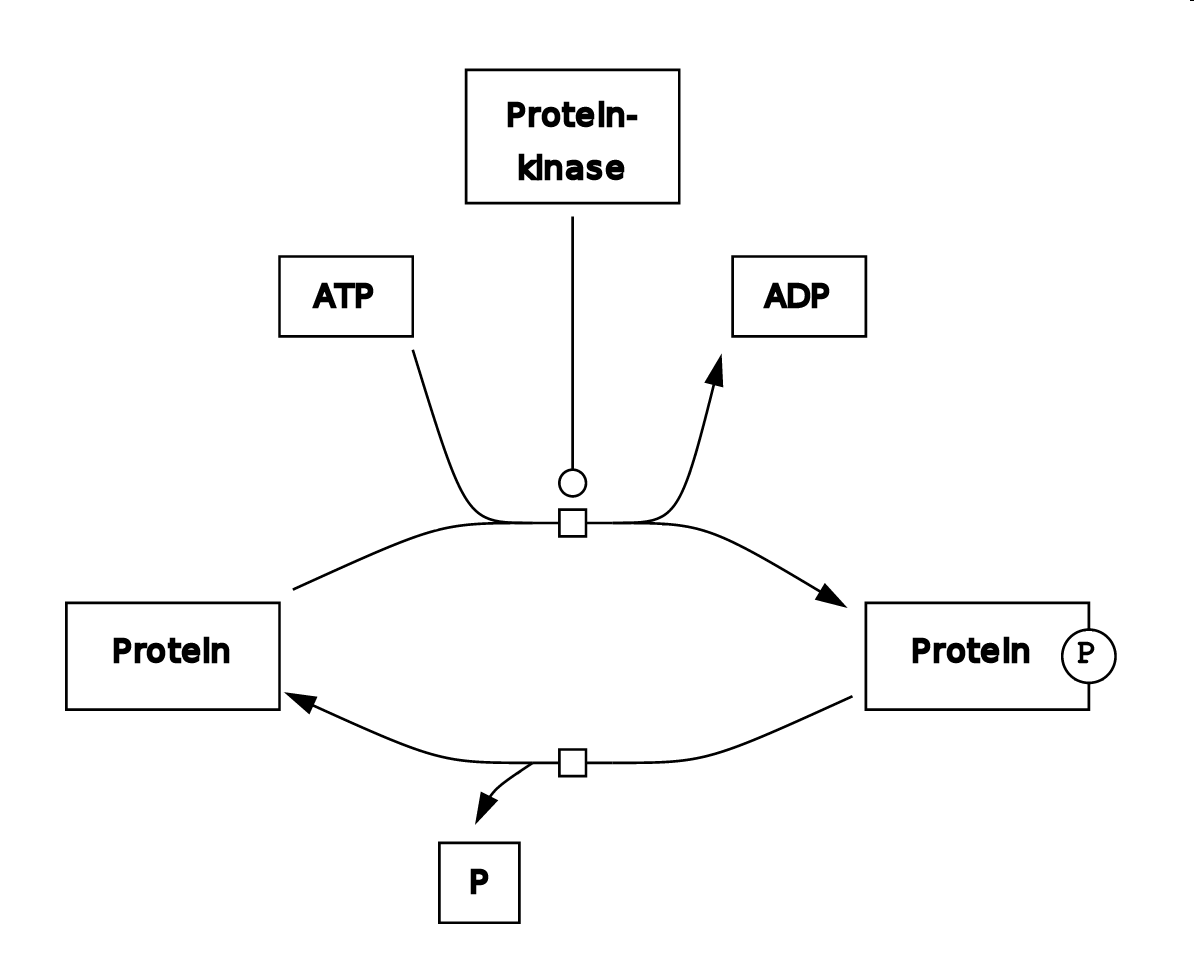
\includegraphics[width=0.4\textwidth]{figures/Phosphorylation_wireFrame}
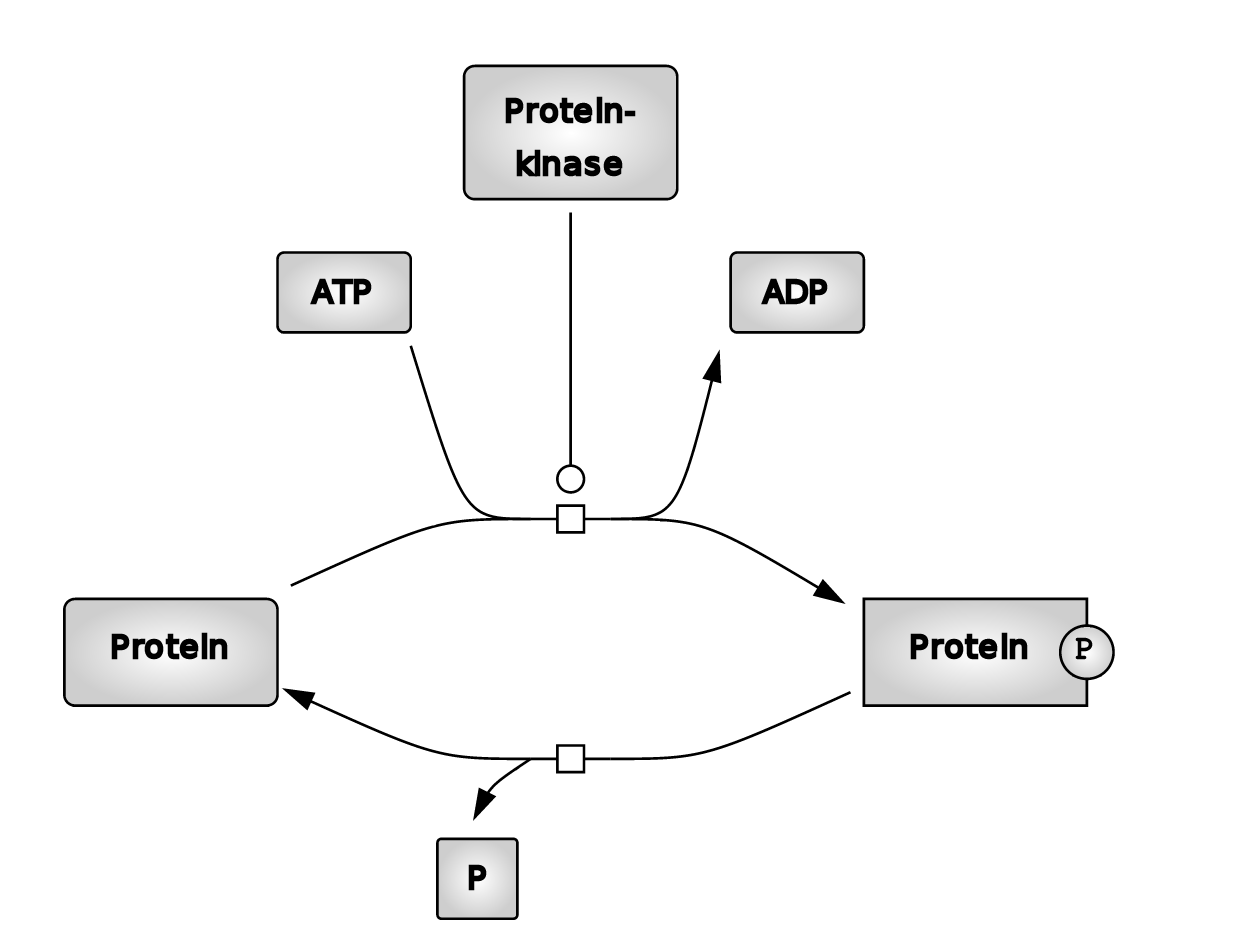
\includegraphics[width=0.4\textwidth]{figures/Phosphorylation_gray}
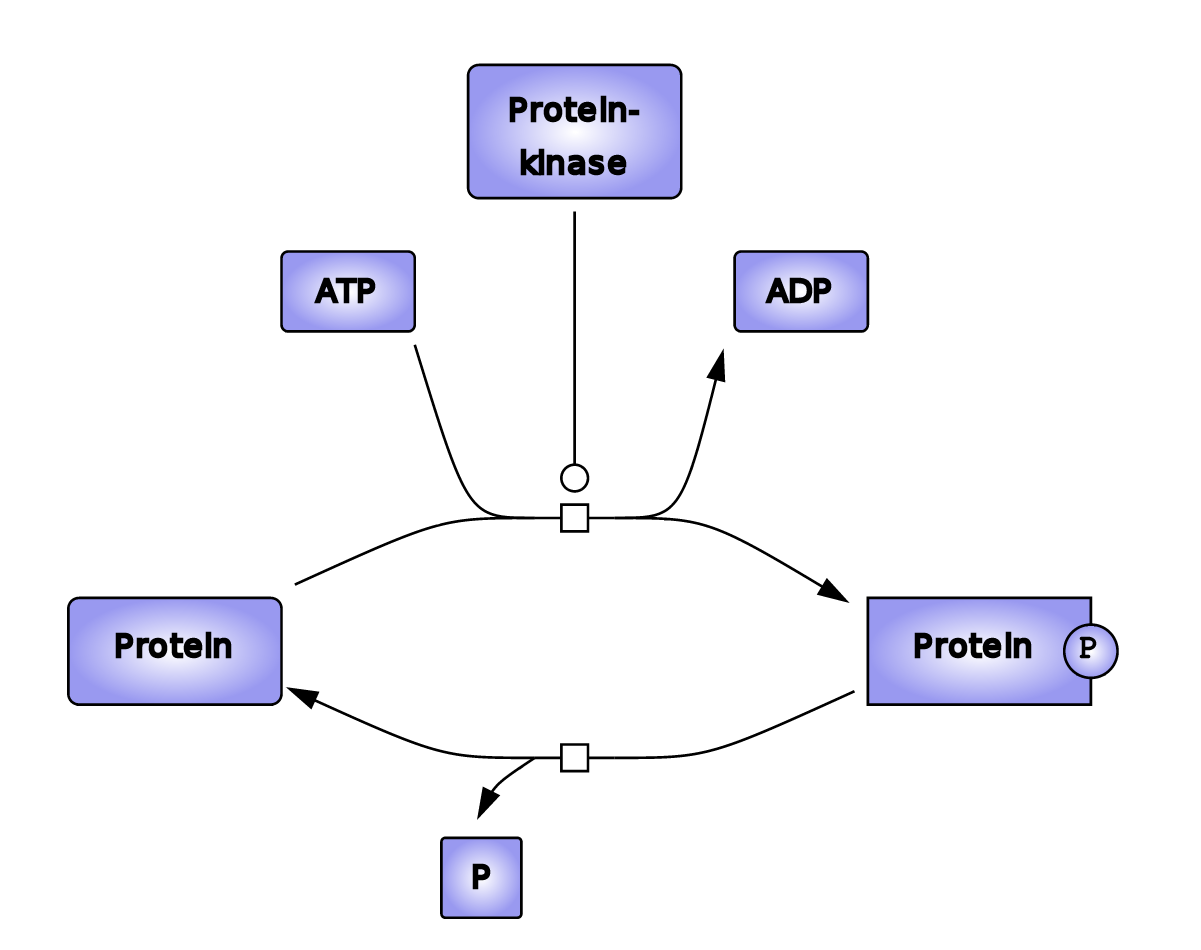
\includegraphics[width=0.4\textwidth]{figures/Phosphorylation_color}
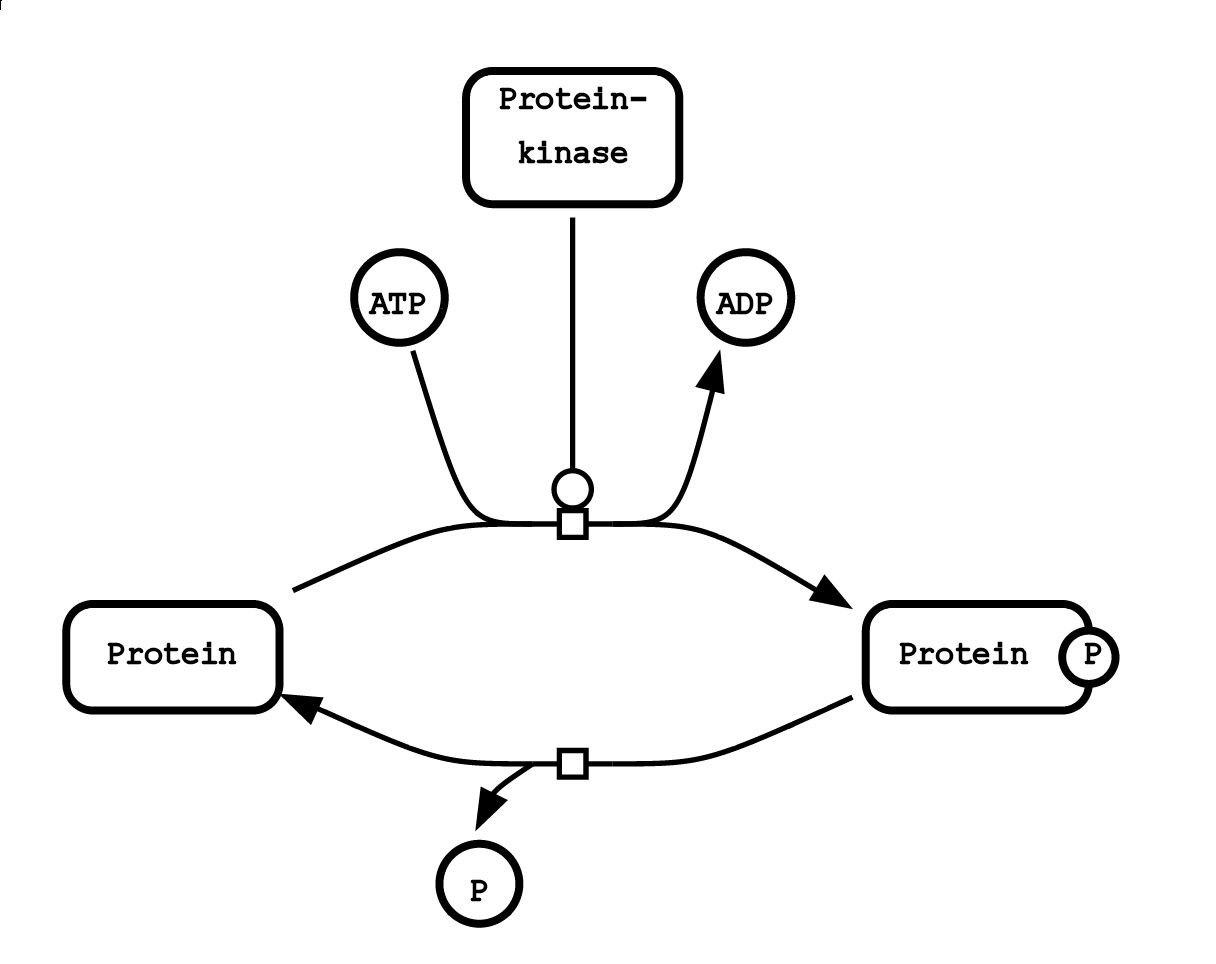
\includegraphics[width=0.4\textwidth]{figures/Phosphorylation_SBGN}
\end{center}
\caption{example converted to SVG and rendered with Google Chrome browser}
\label{ExampleRendering}
\end{figure}

